\setchapterstyle{lines}
\labch{appendix}

\setchapterstyle{lines}
\chapter{Heavy Neutral Lepton Signal Simulation}
\labch{signal_simulation_appenix}


\section{Model Independent Simulation Distributions} \labsec{model_independent_simulation_appendix}

\begin{figure*}[h]
    \centering
    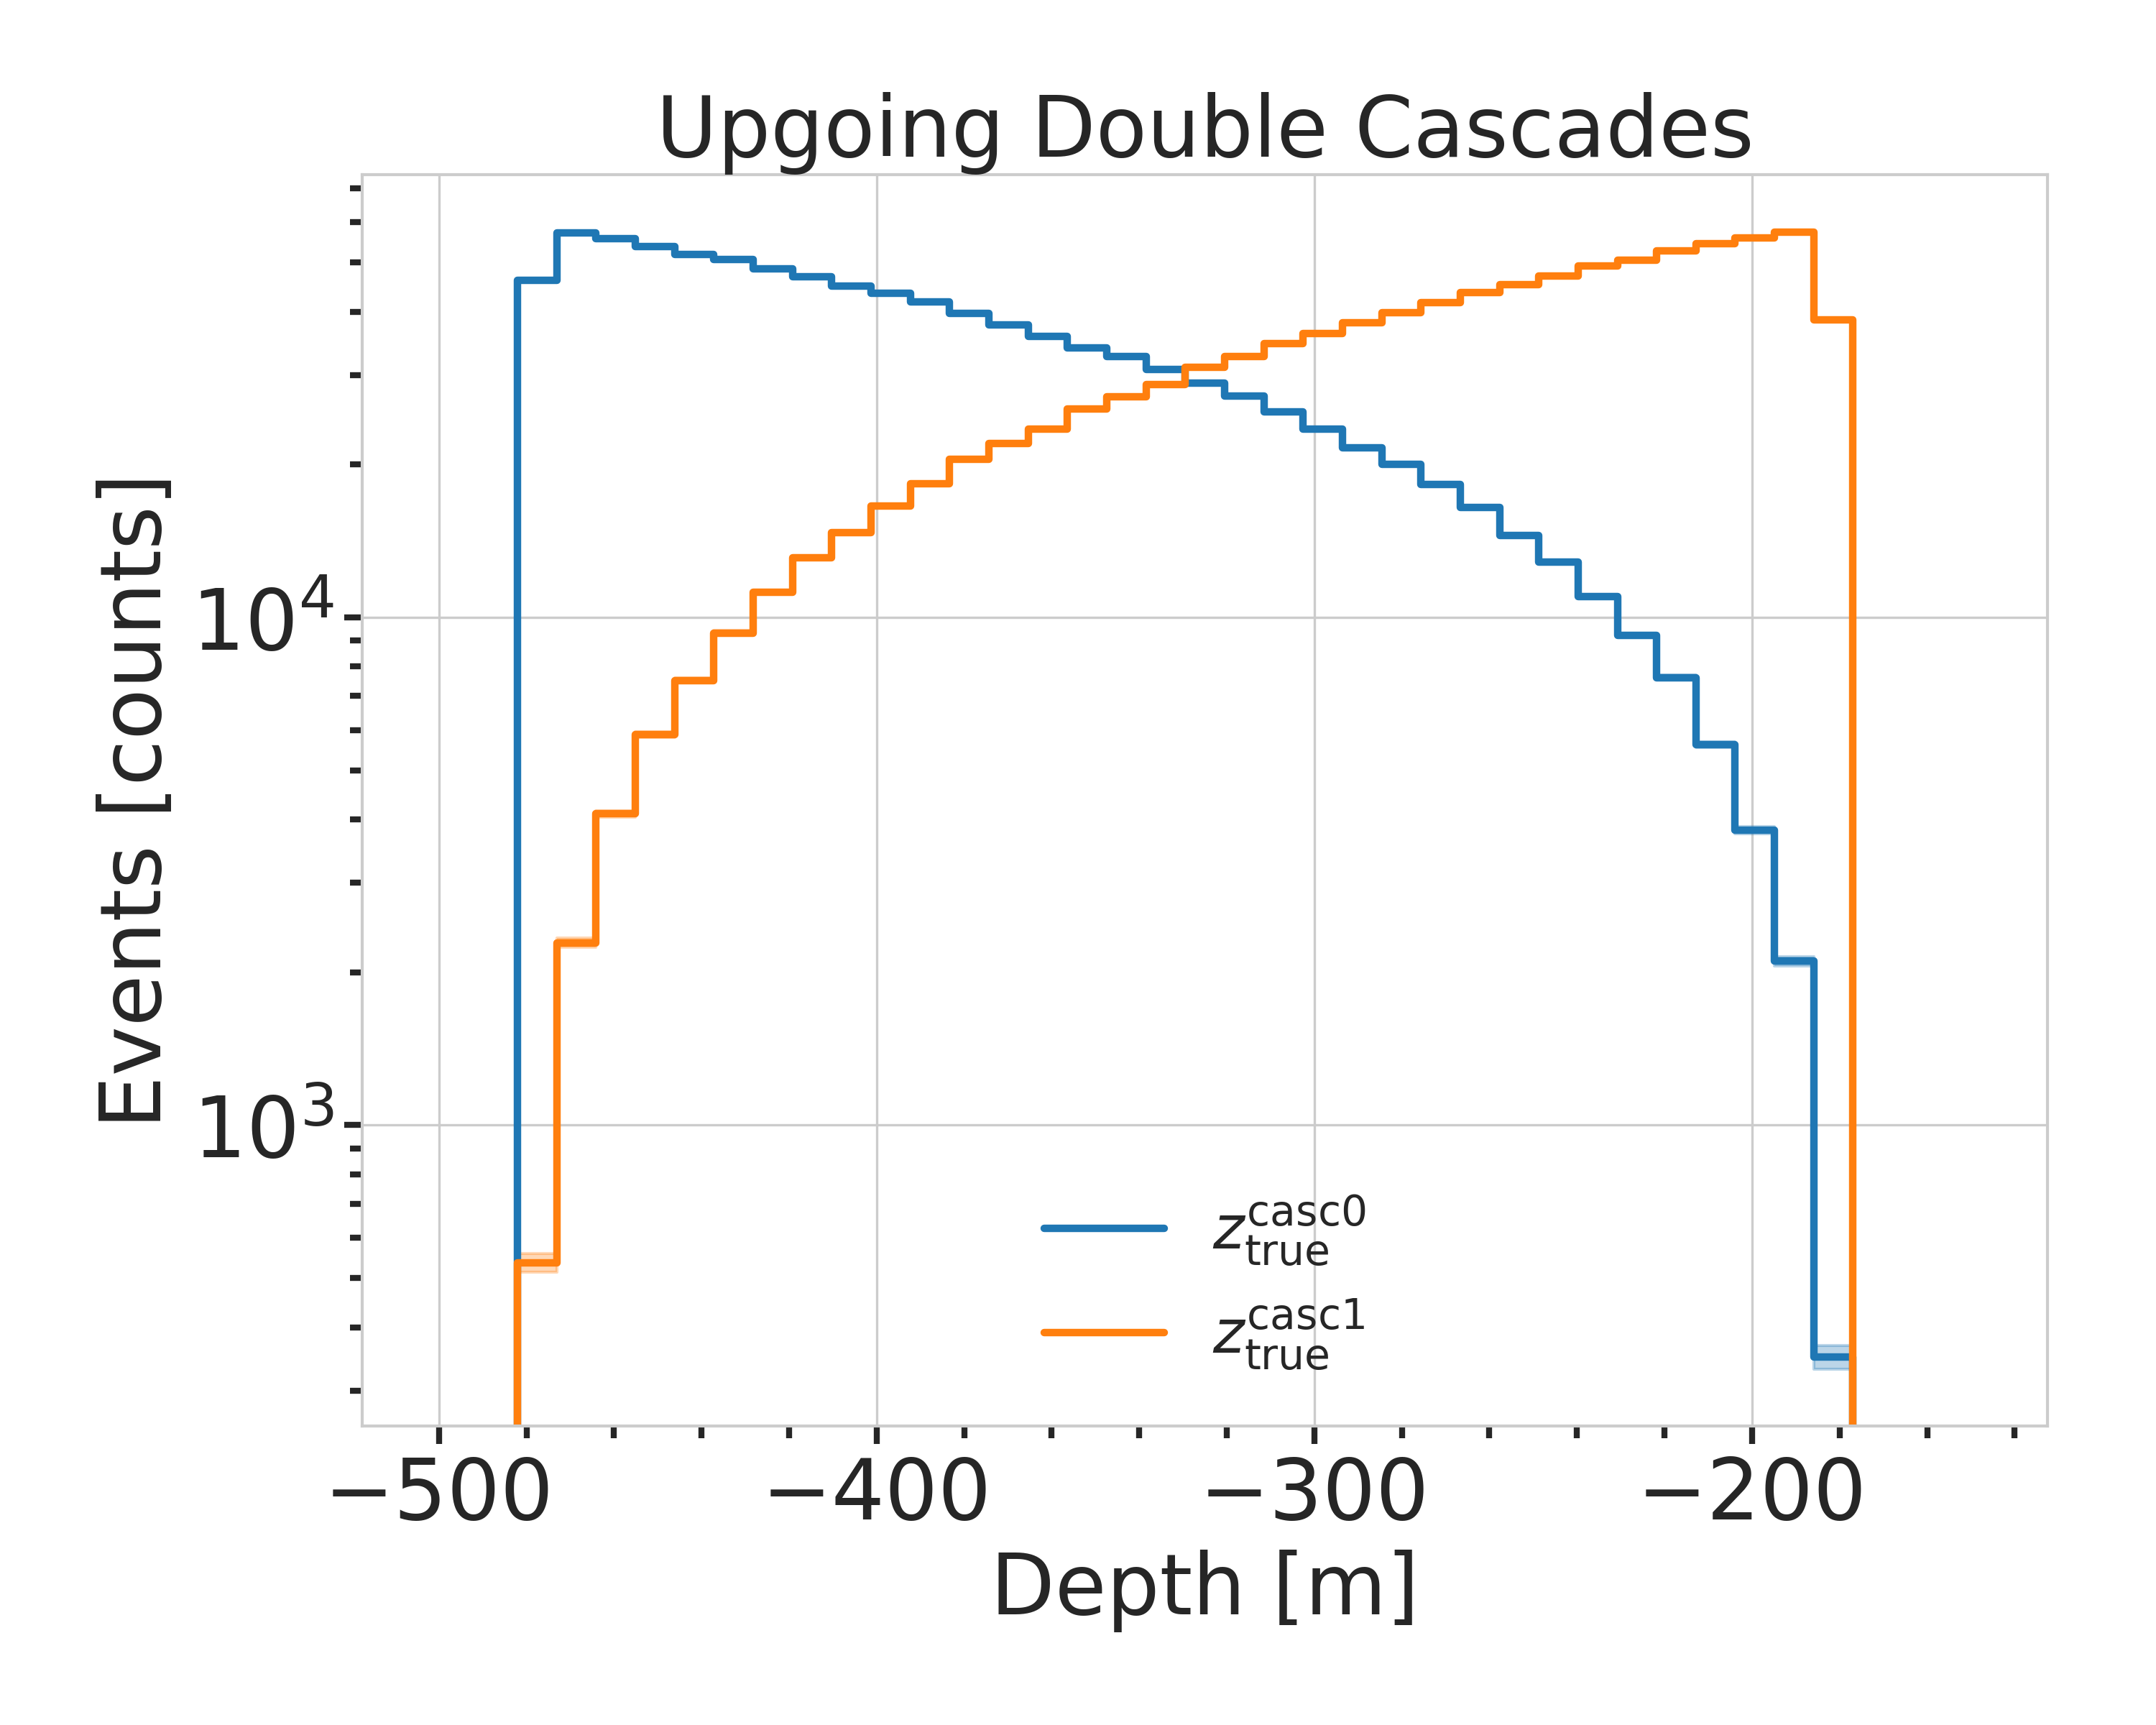
\includegraphics[width=0.49\linewidth]{figures/model_independent_simulation/gen_level/1_d_distr_depths_clipped.png}
    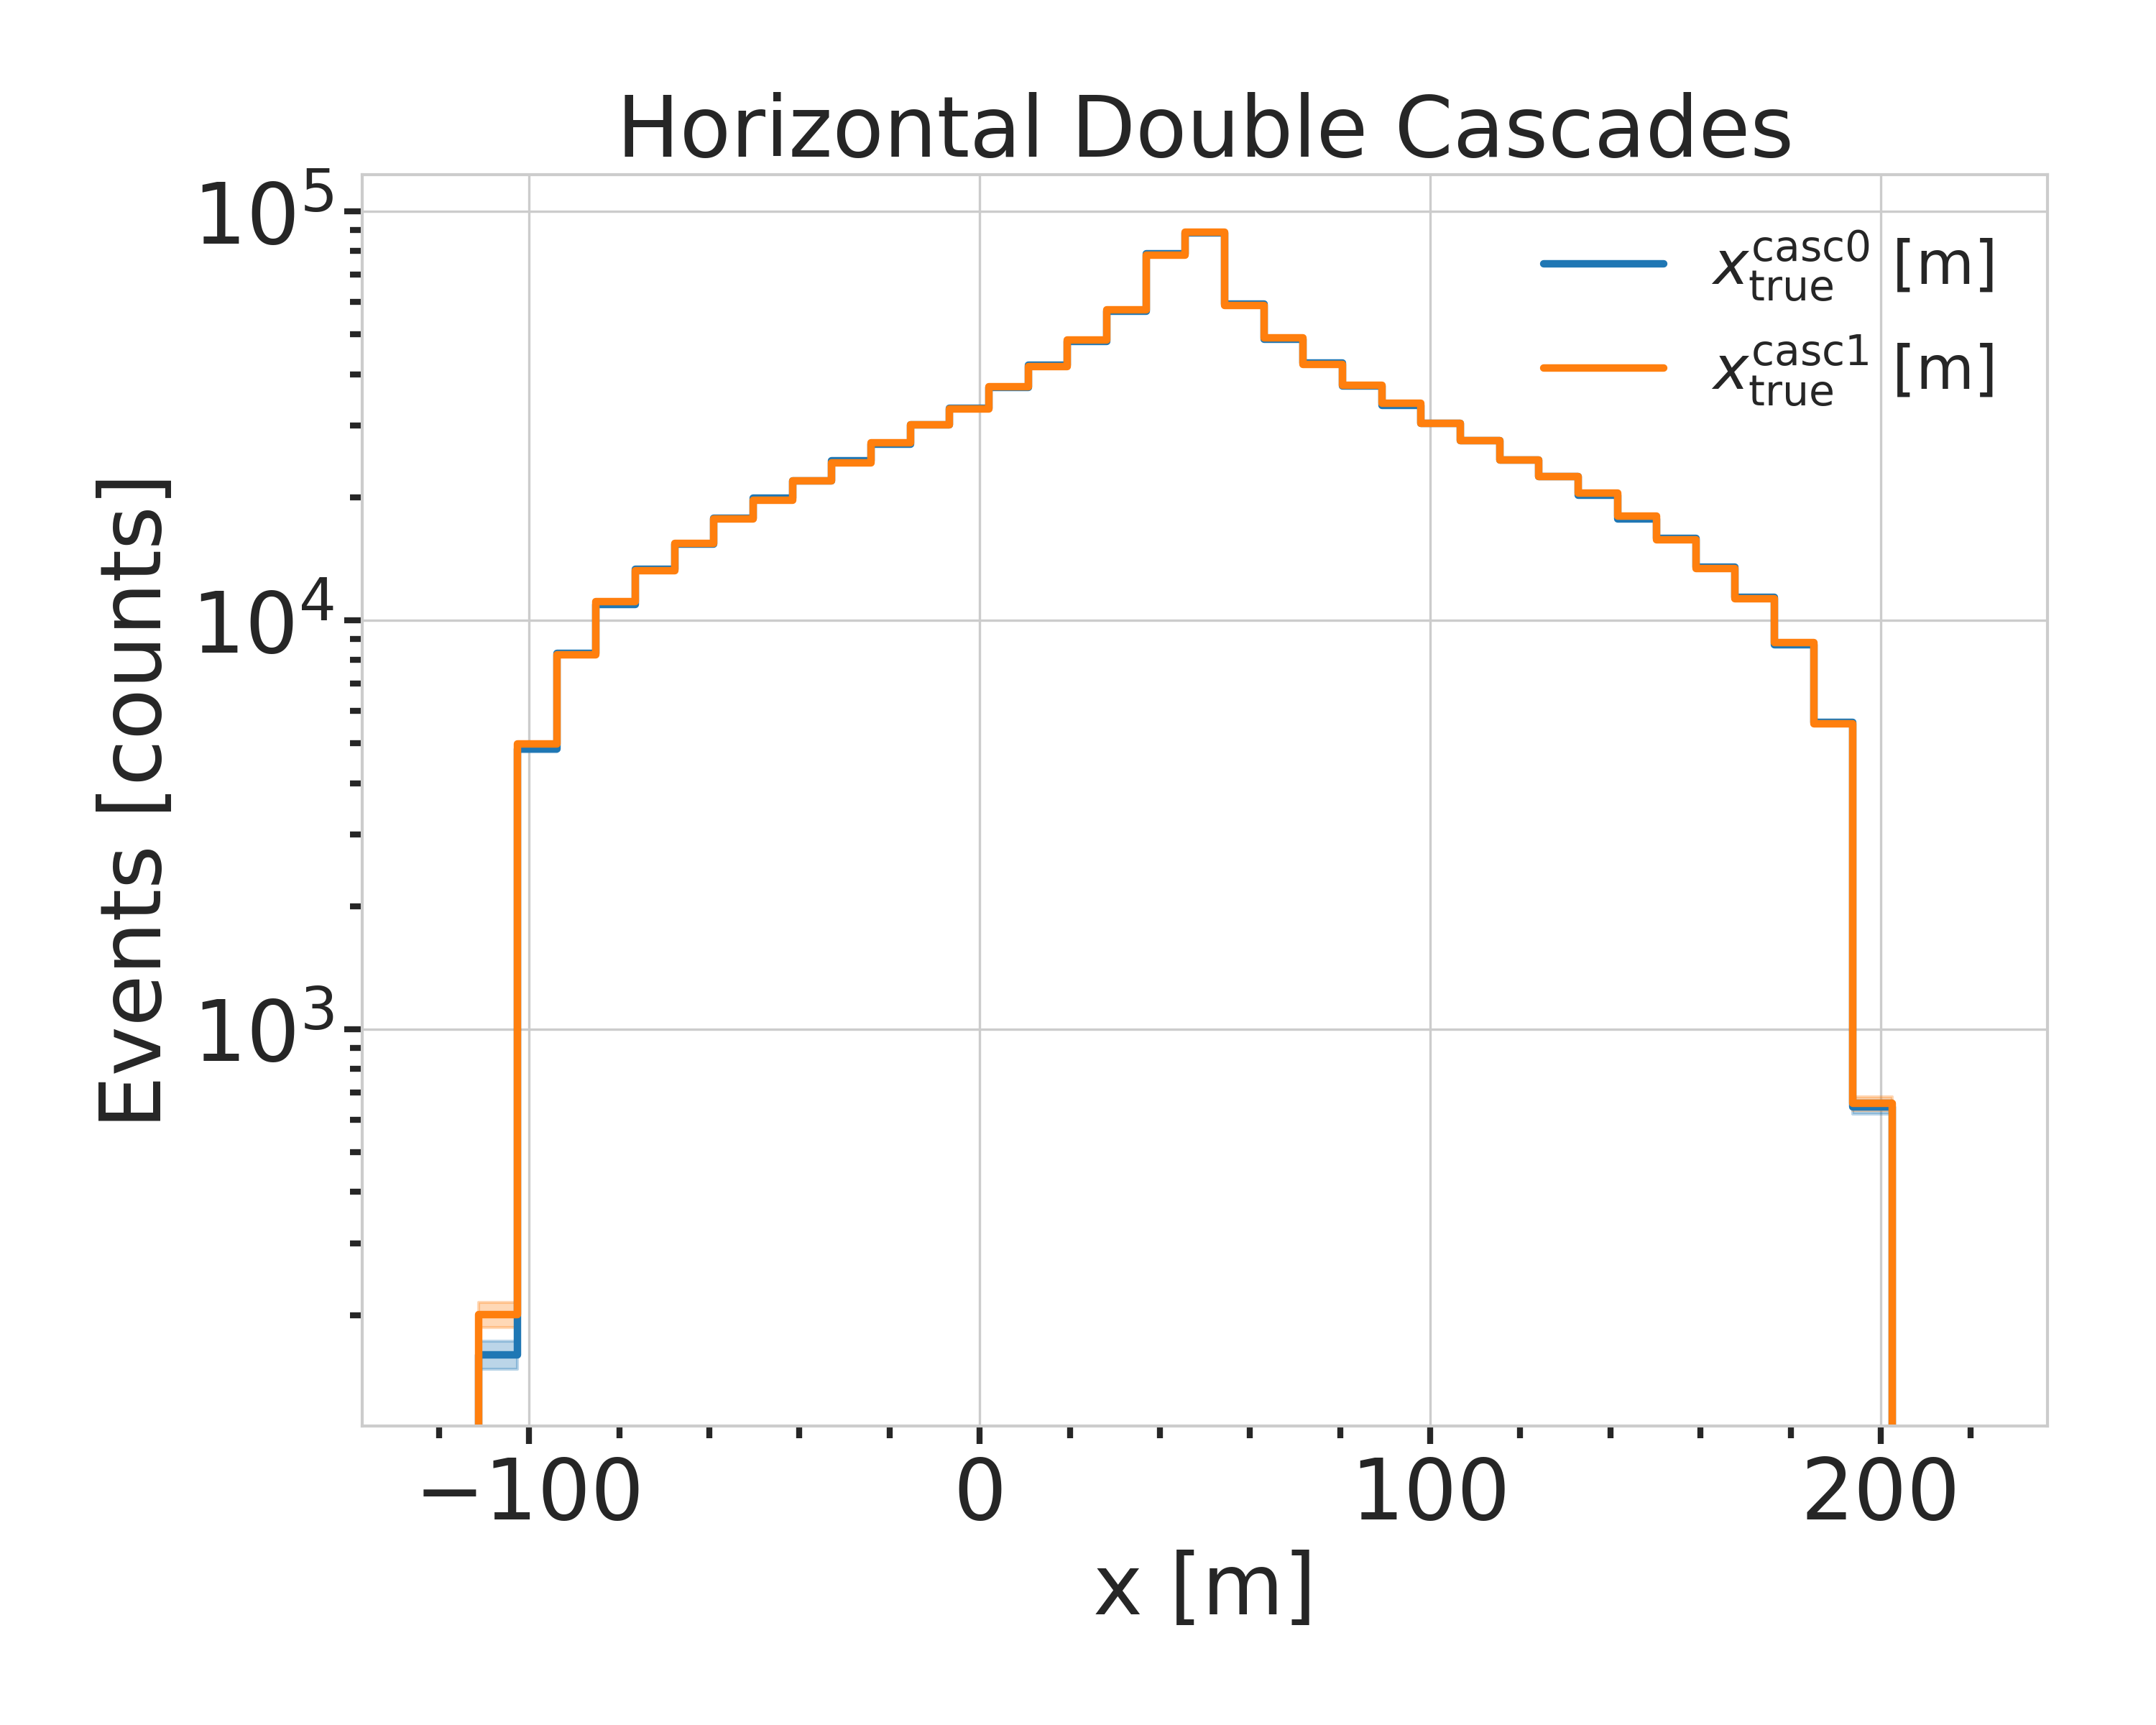
\includegraphics[width=0.49\linewidth]{figures/model_independent_simulation/gen_level/1_d_distr_xs_clipped.png}
    \caption[Simplified model independent simulation generation level distributions]{Generation level distributions of the simplistic simulation sets. Vertical positions (left) and horizontal positions (right) of both sets are shown.}
    \labfig{simplified_gen_distris_appendix}
\end{figure*}

\todo{Re-make plot with x,y for horizontal set one plot!}

\begin{figure*}
    \centering
    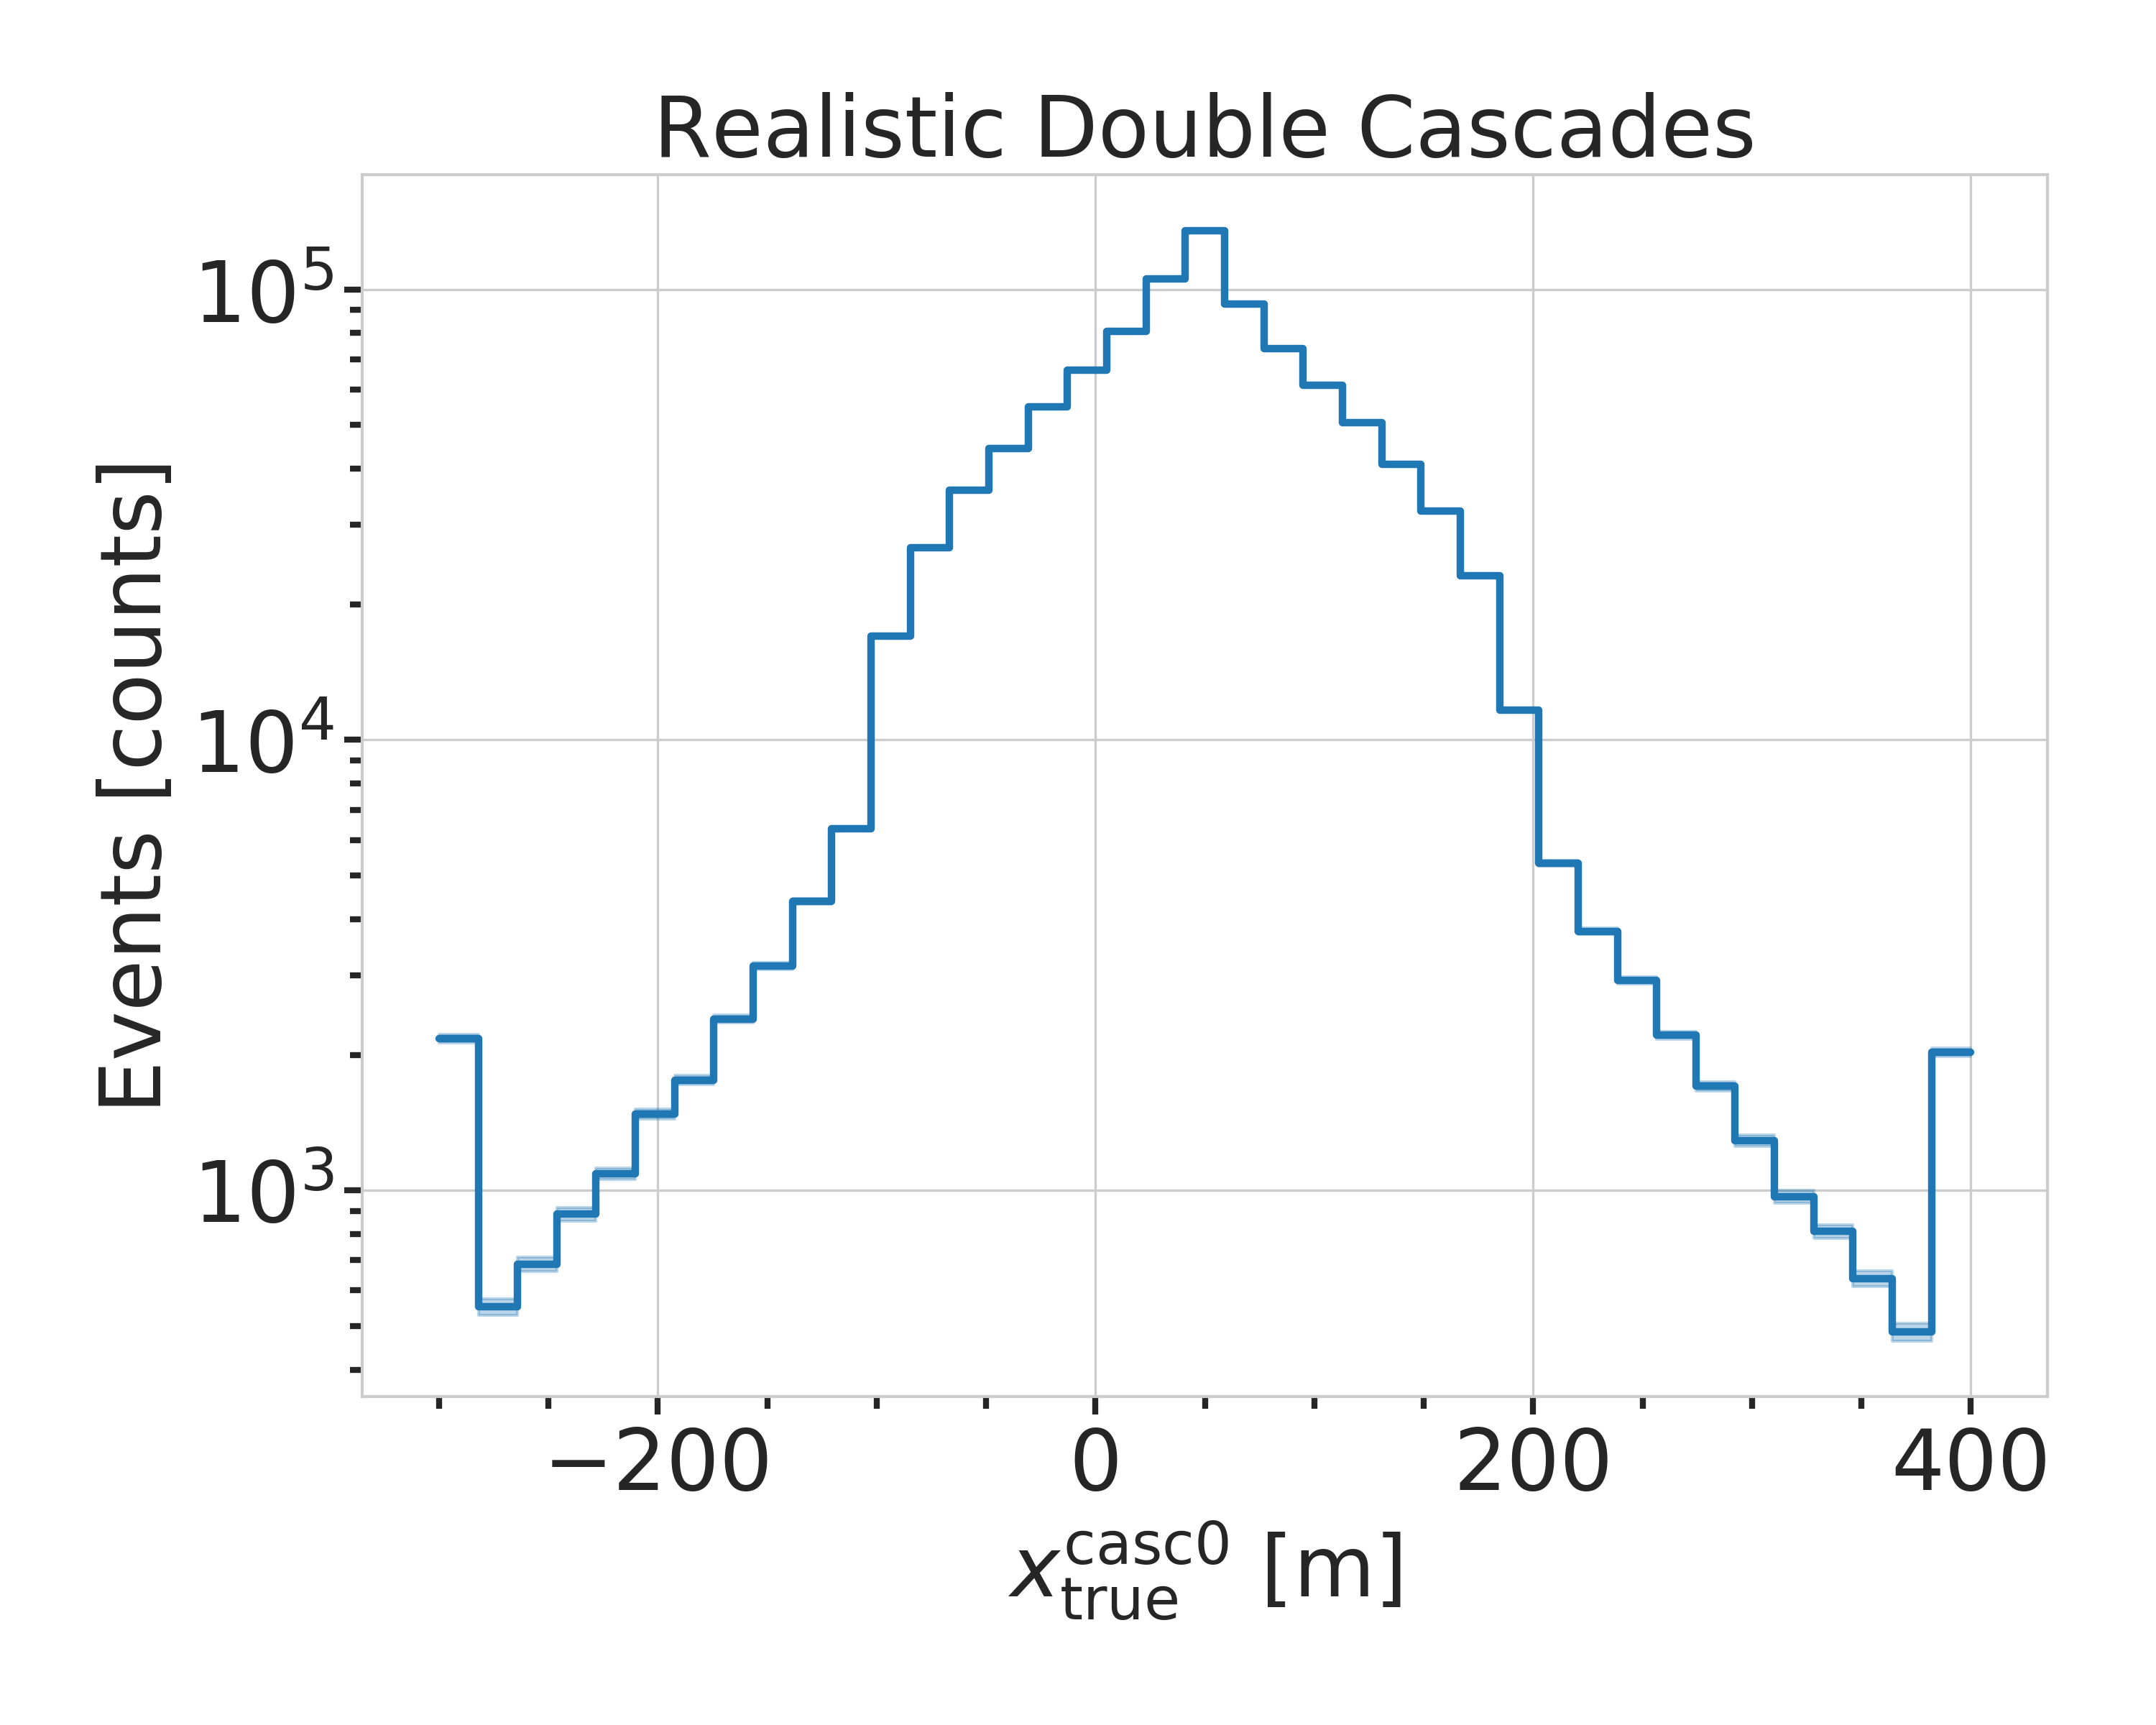
\includegraphics[width=0.49\linewidth]{figures/model_independent_simulation/gen_level/194603_gen_level_1_d_distr_casc0_true_x_clipped.png}
    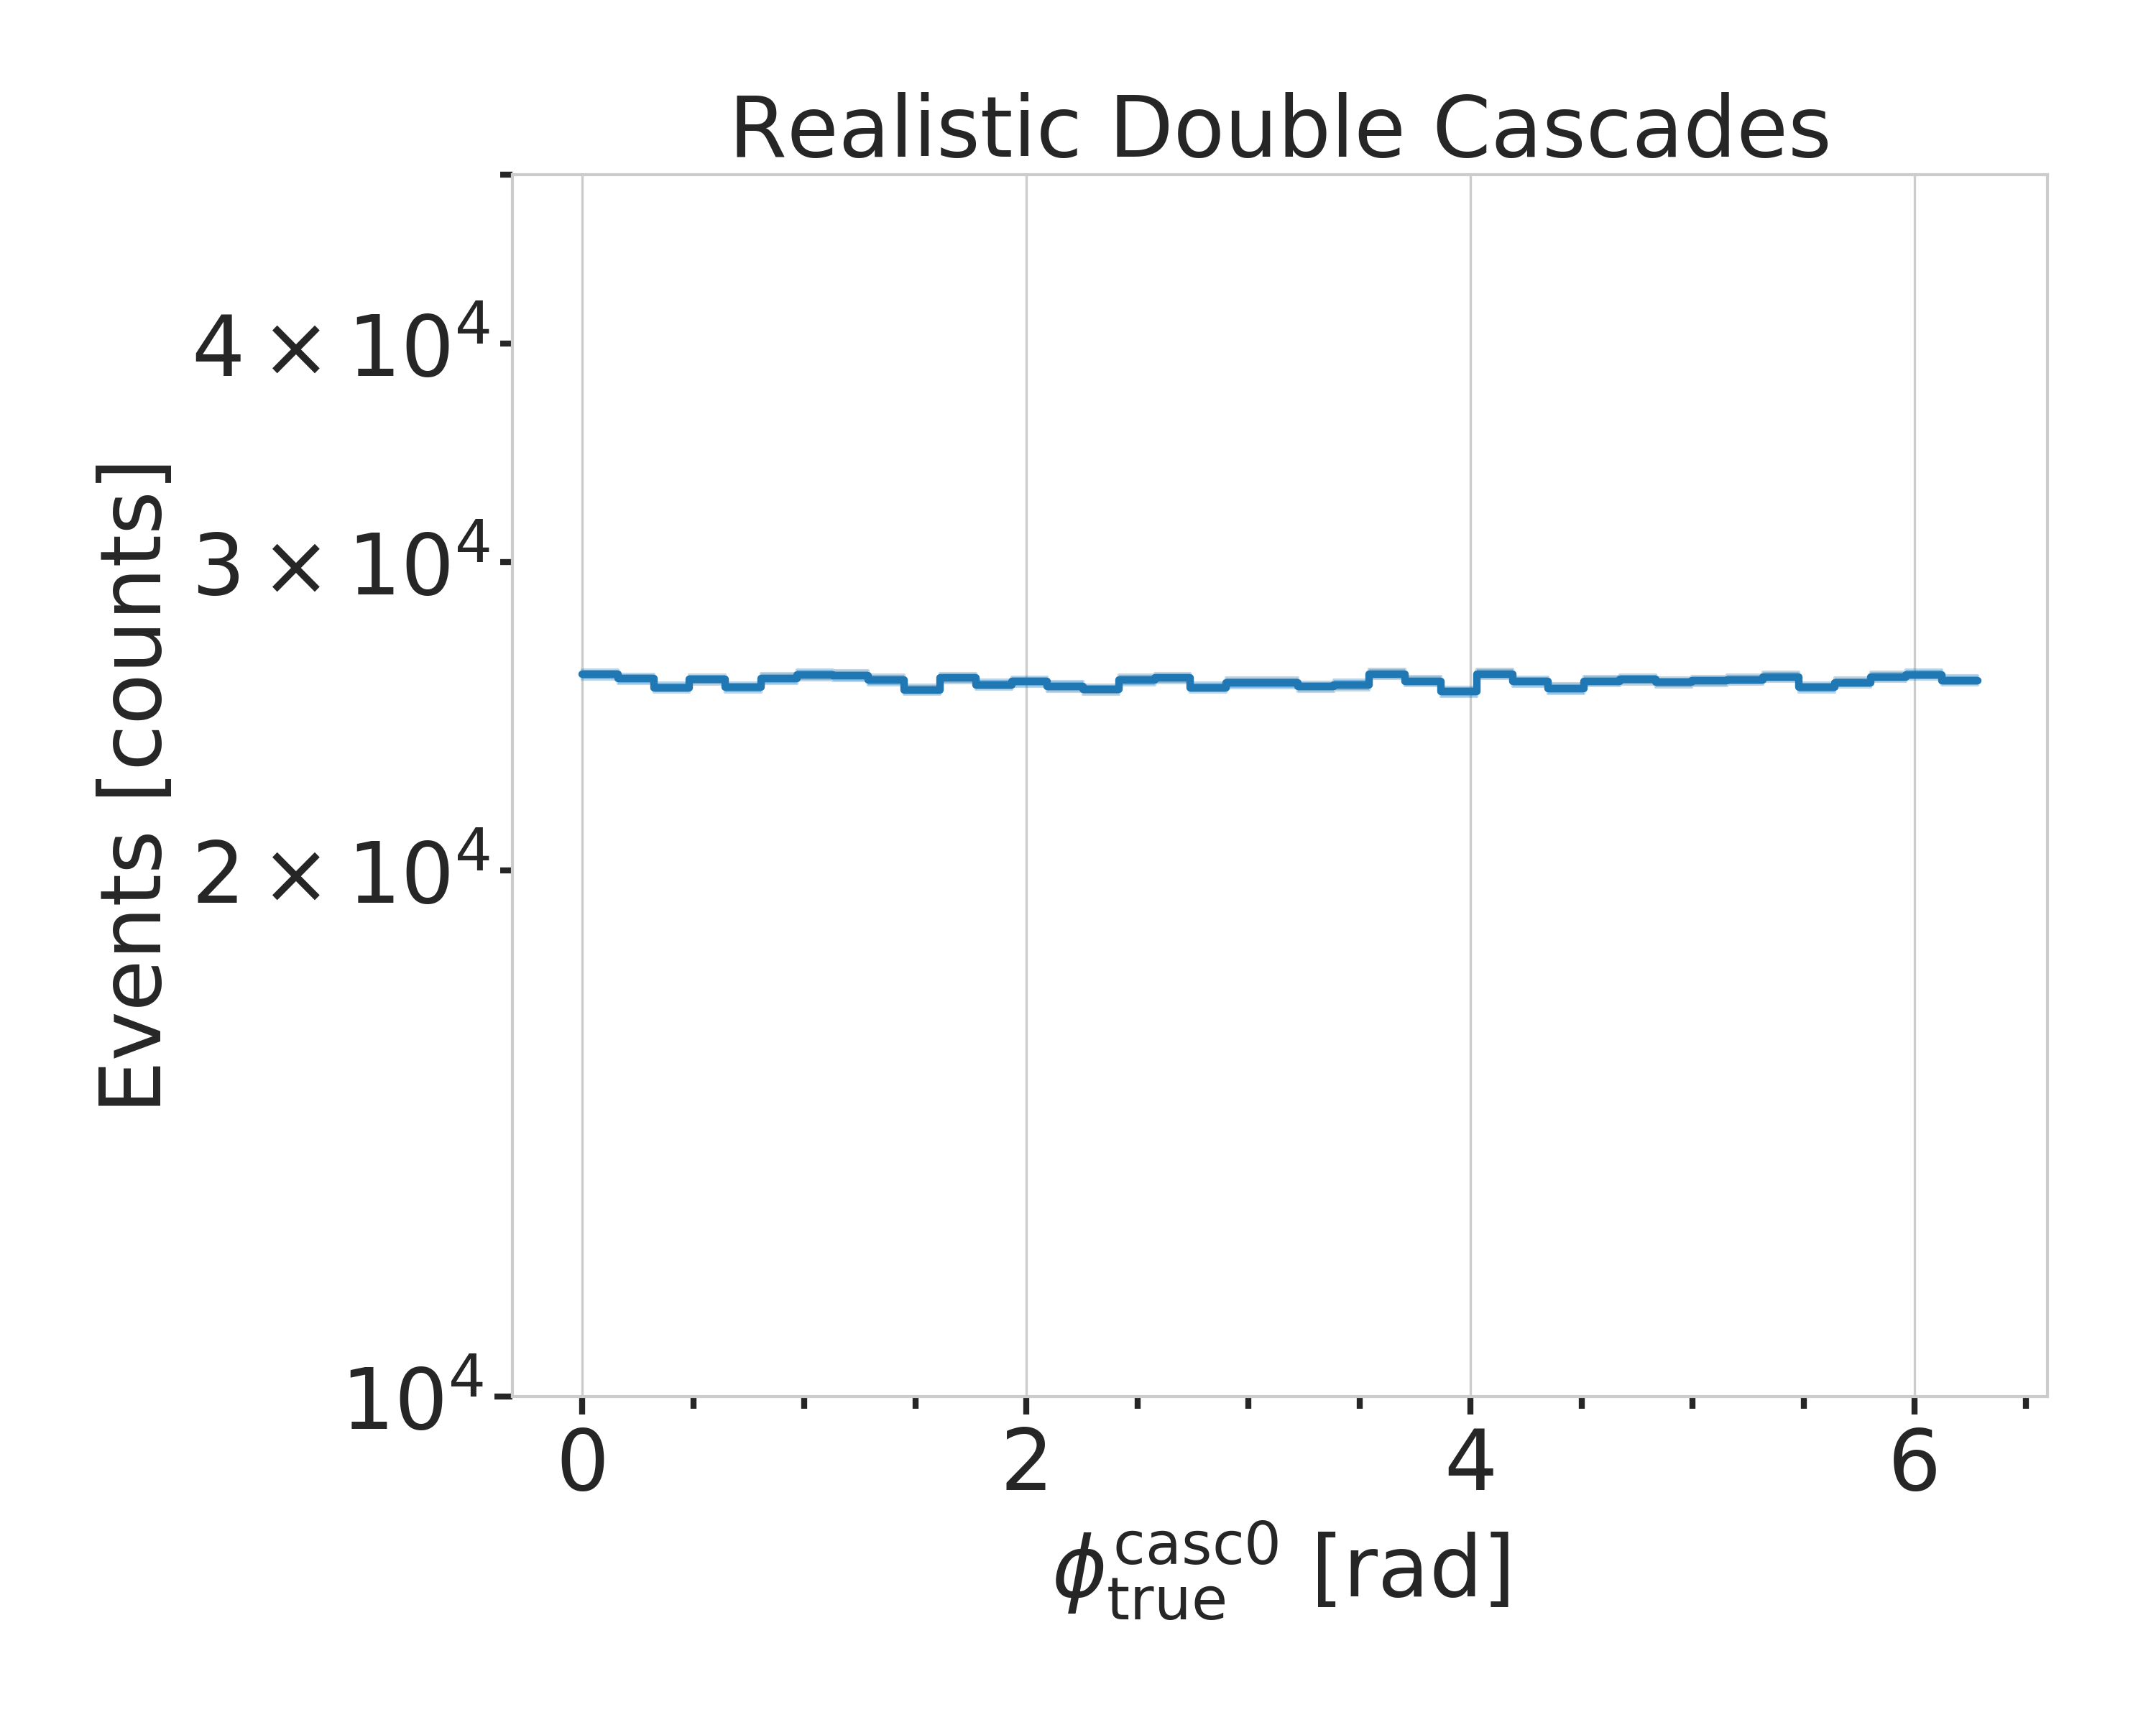
\includegraphics[width=0.49\linewidth]{figures/model_independent_simulation/gen_level/194603_gen_level_1_d_distr_casc0_true_azimuth_clipped.png}
    \caption[Realistic model independent simulation generation level distributions]{Generation level distributions of the realistic simulation set. Shown are the cascade $x, y, z$ positions (left) and direction angles (right).}
    \labfig{realistic_gen_distris_appendix}
\end{figure*}

\todo{Re-make plot with x, y, z for both cascades in one.}
\todo{Re-arrange plots in a more sensible way.}


\section{Model Dependent Simulation Distributions} \labsec{model_dependent_simulation_appendix}

\begin{figure*}[h]
    \centering
    \begin{subfigure}{0.49\linewidth}
        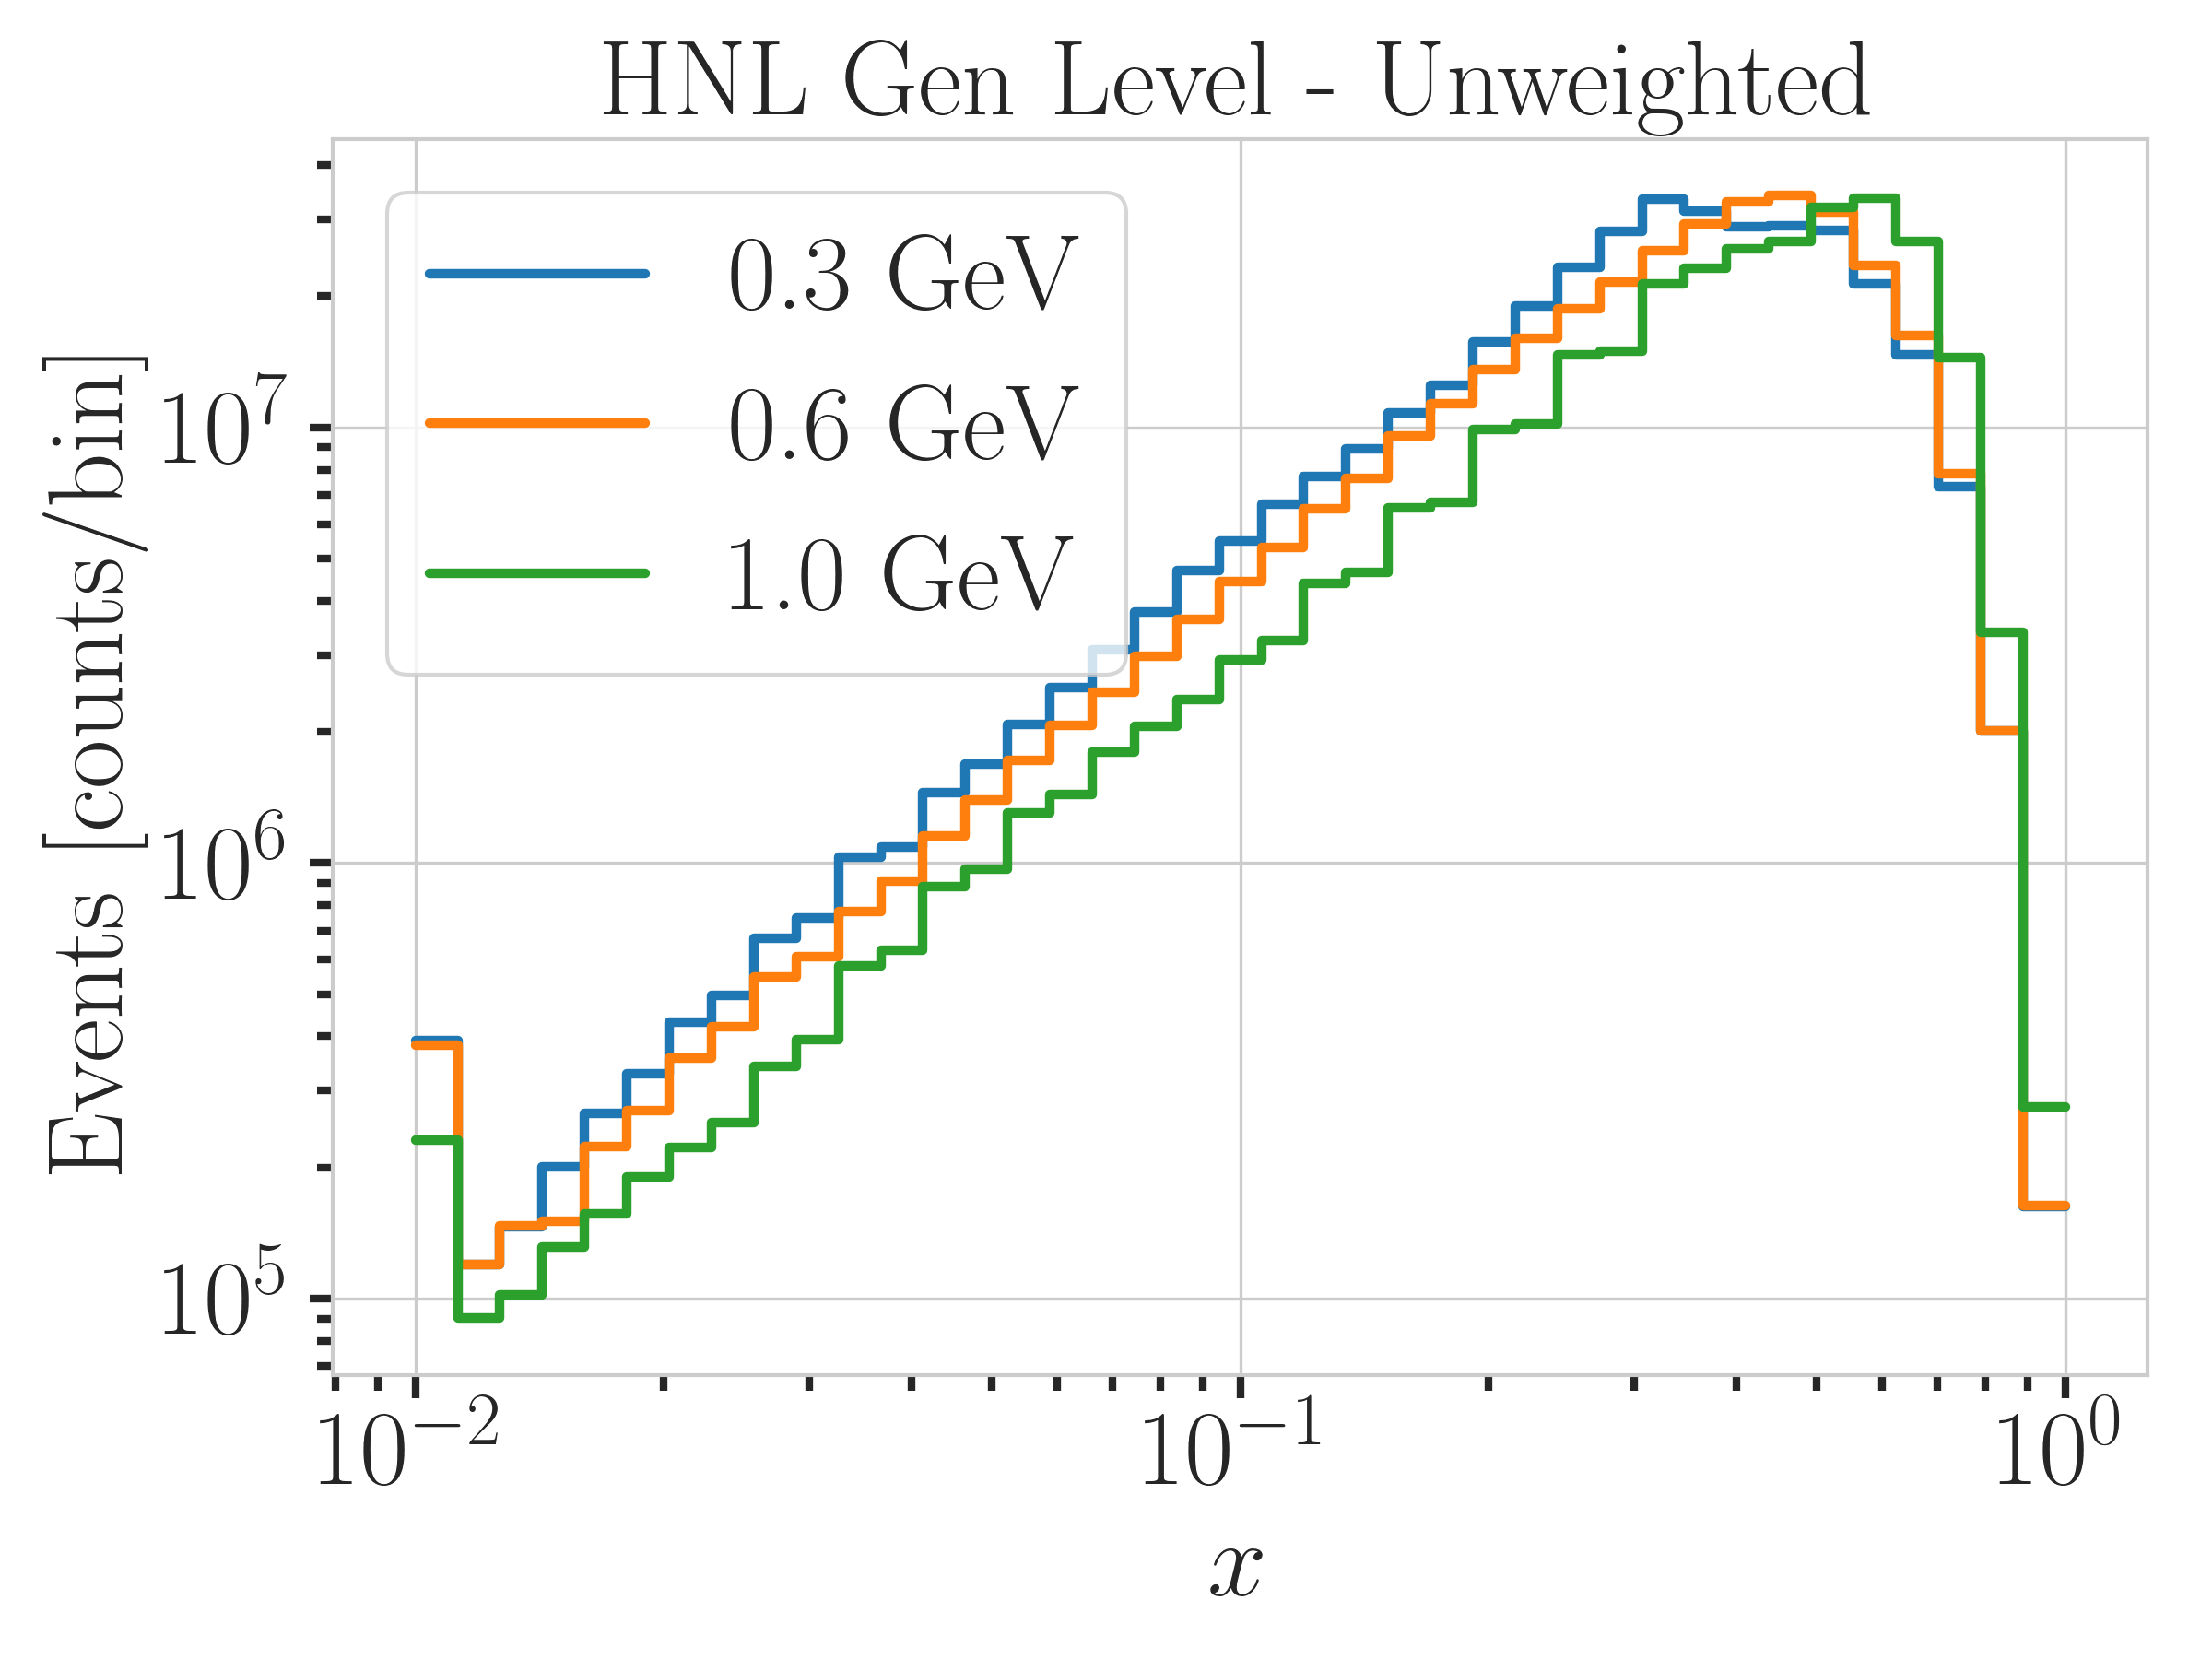
\includegraphics{figures/hnl_simulation/generation/1_d_distr_finalStateX_gen_level_unweighted.png}
        \caption{Bjorken x}
    \end{subfigure}
    \begin{subfigure}{0.49\linewidth}
    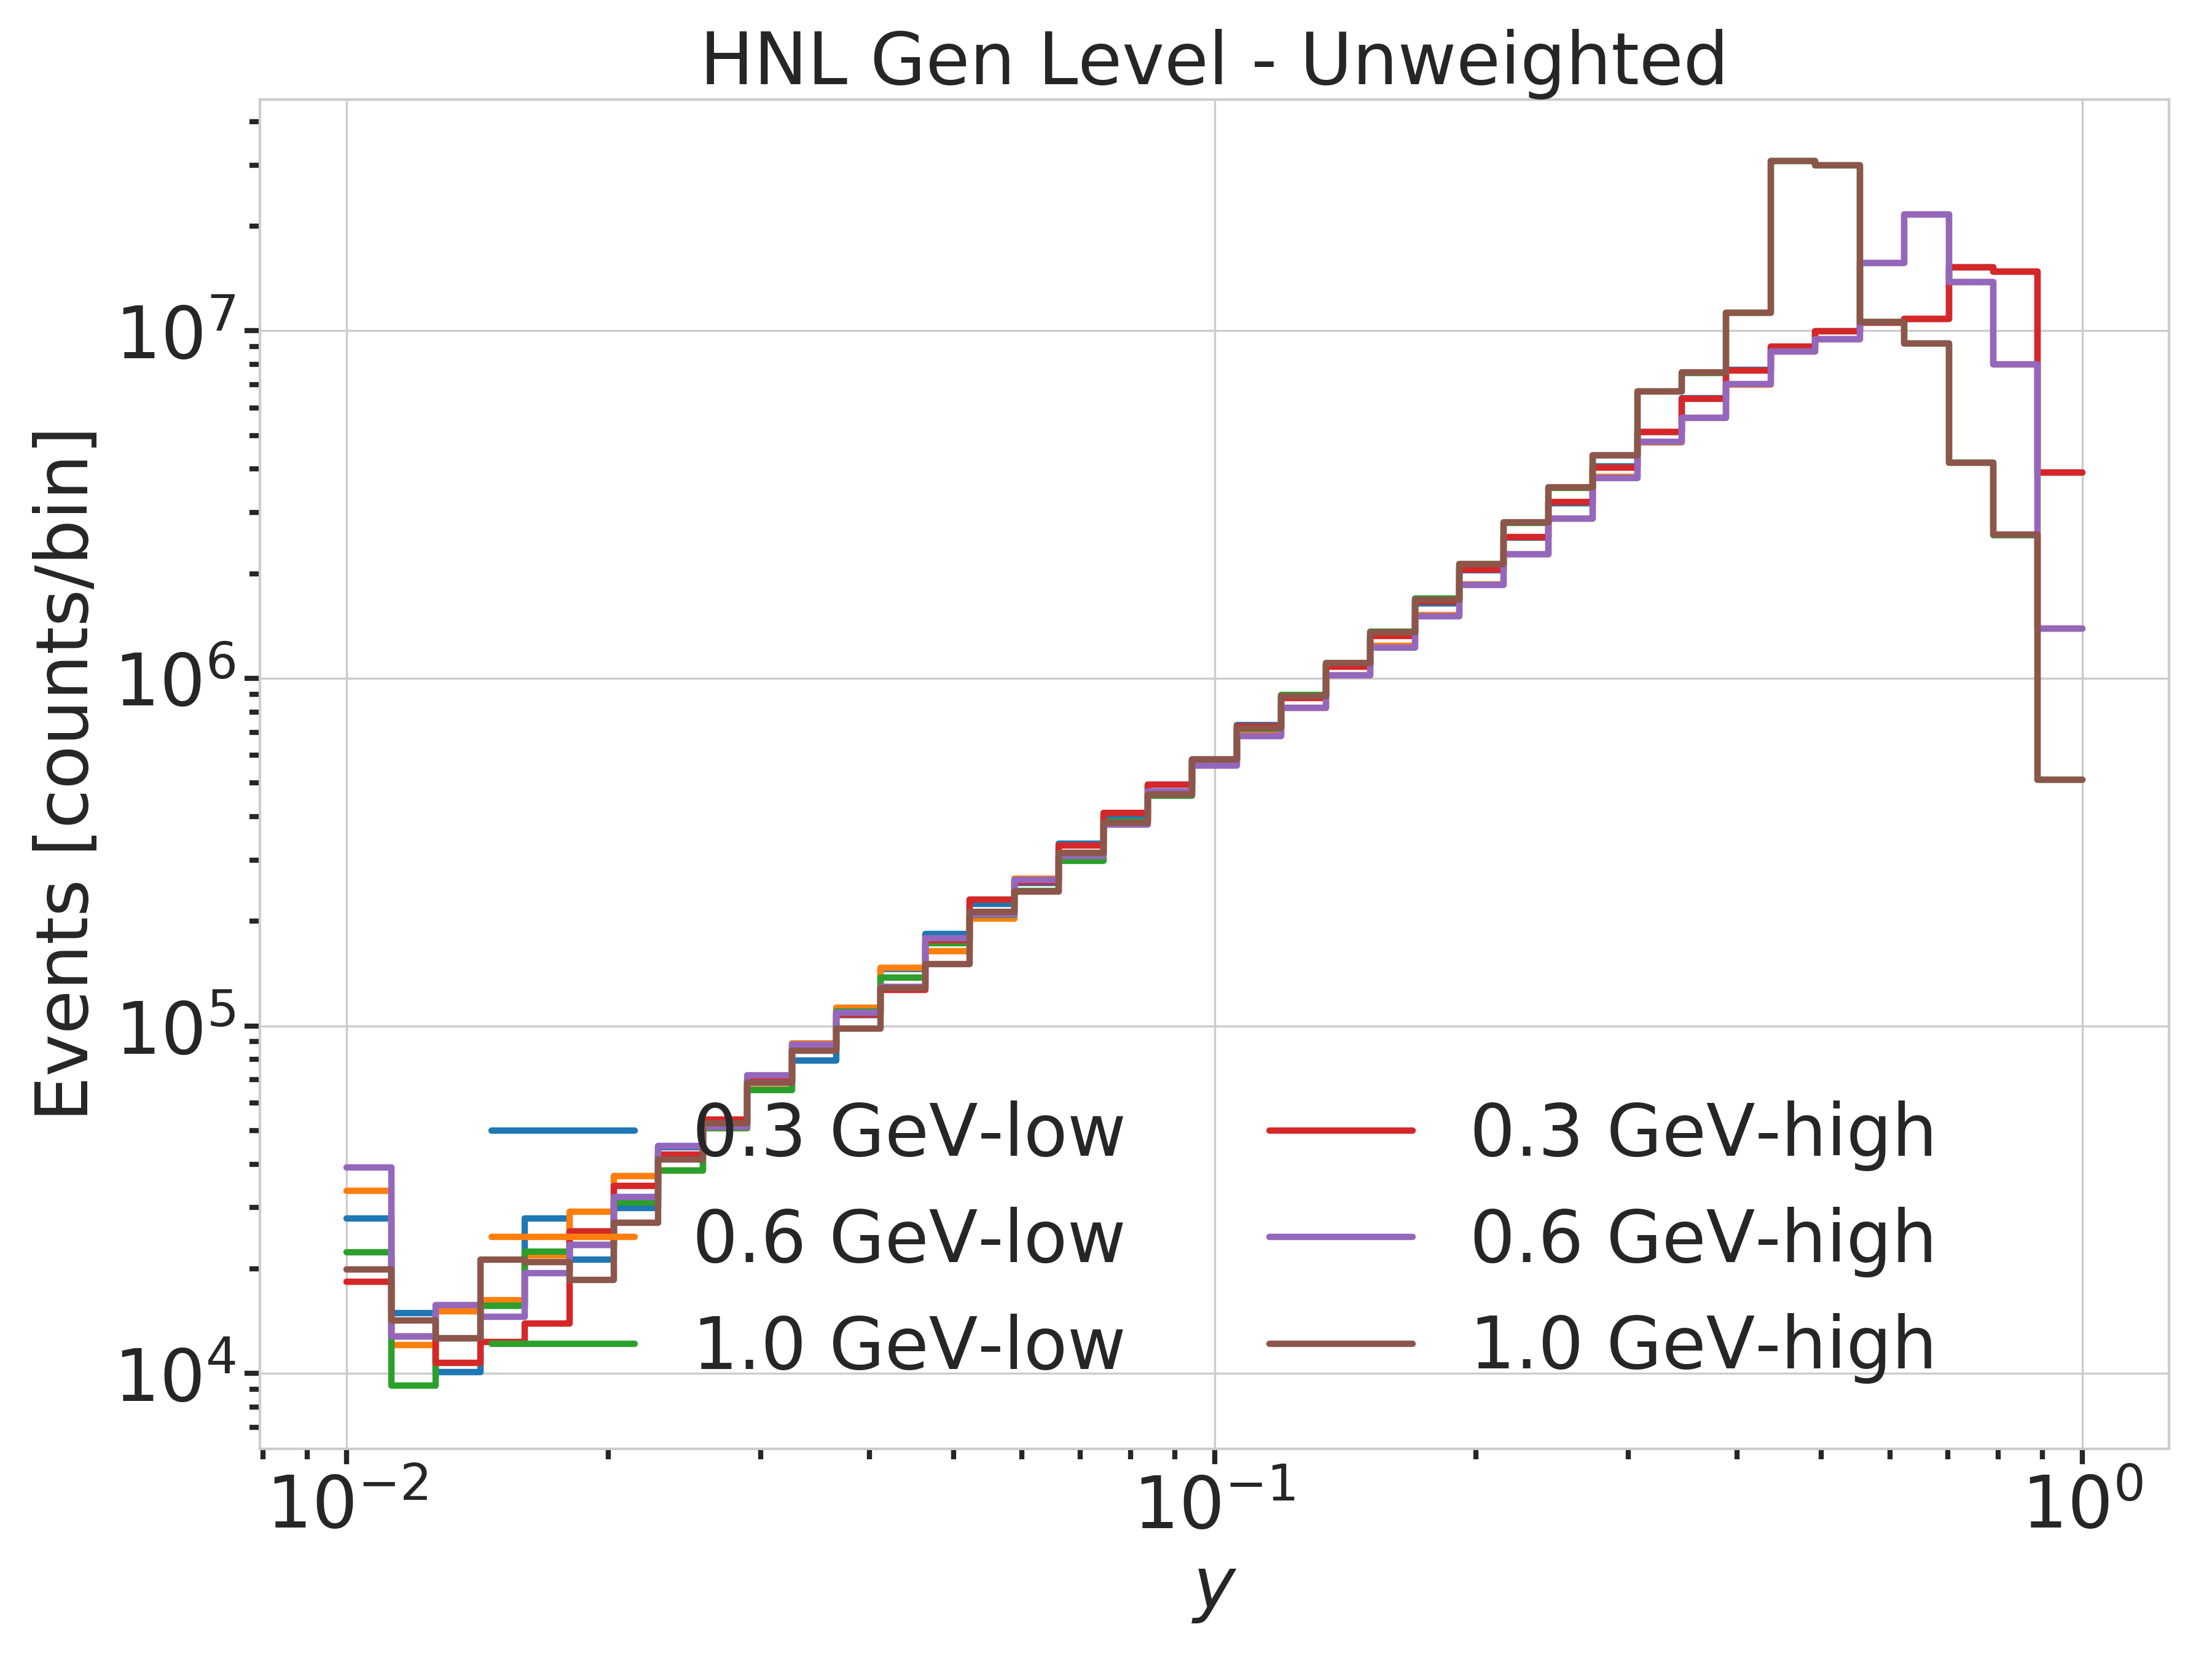
\includegraphics{figures/hnl_simulation/generation/1_d_distr_finalStateY_gen_level_unweighted.png}
        \caption{Bjorken y}
    \end{subfigure}
    \caption[Model dependent simulation generation level distributions]{Generation level distributions of the model dependent simulation.}
    \labfig{hnl_gen_distris_appendix}
\end{figure*}


% \setchapterstyle{lines}
% \chapter{Analysis Checks}
% \labch{analysis_checks}


% \section{Minimization Robustness} \labsec{asimov_inject_recover_appendix}

% \reffig{asimov_inject_recover_appendix} shows additional Asimov inject/recover tests for the \SI{0.3}{\gev} and the \SI{1.0}{\gev} mass sets. The tests were described in \refsec{asimov_inject_recover}.

% \begin{figure*}[h]
%     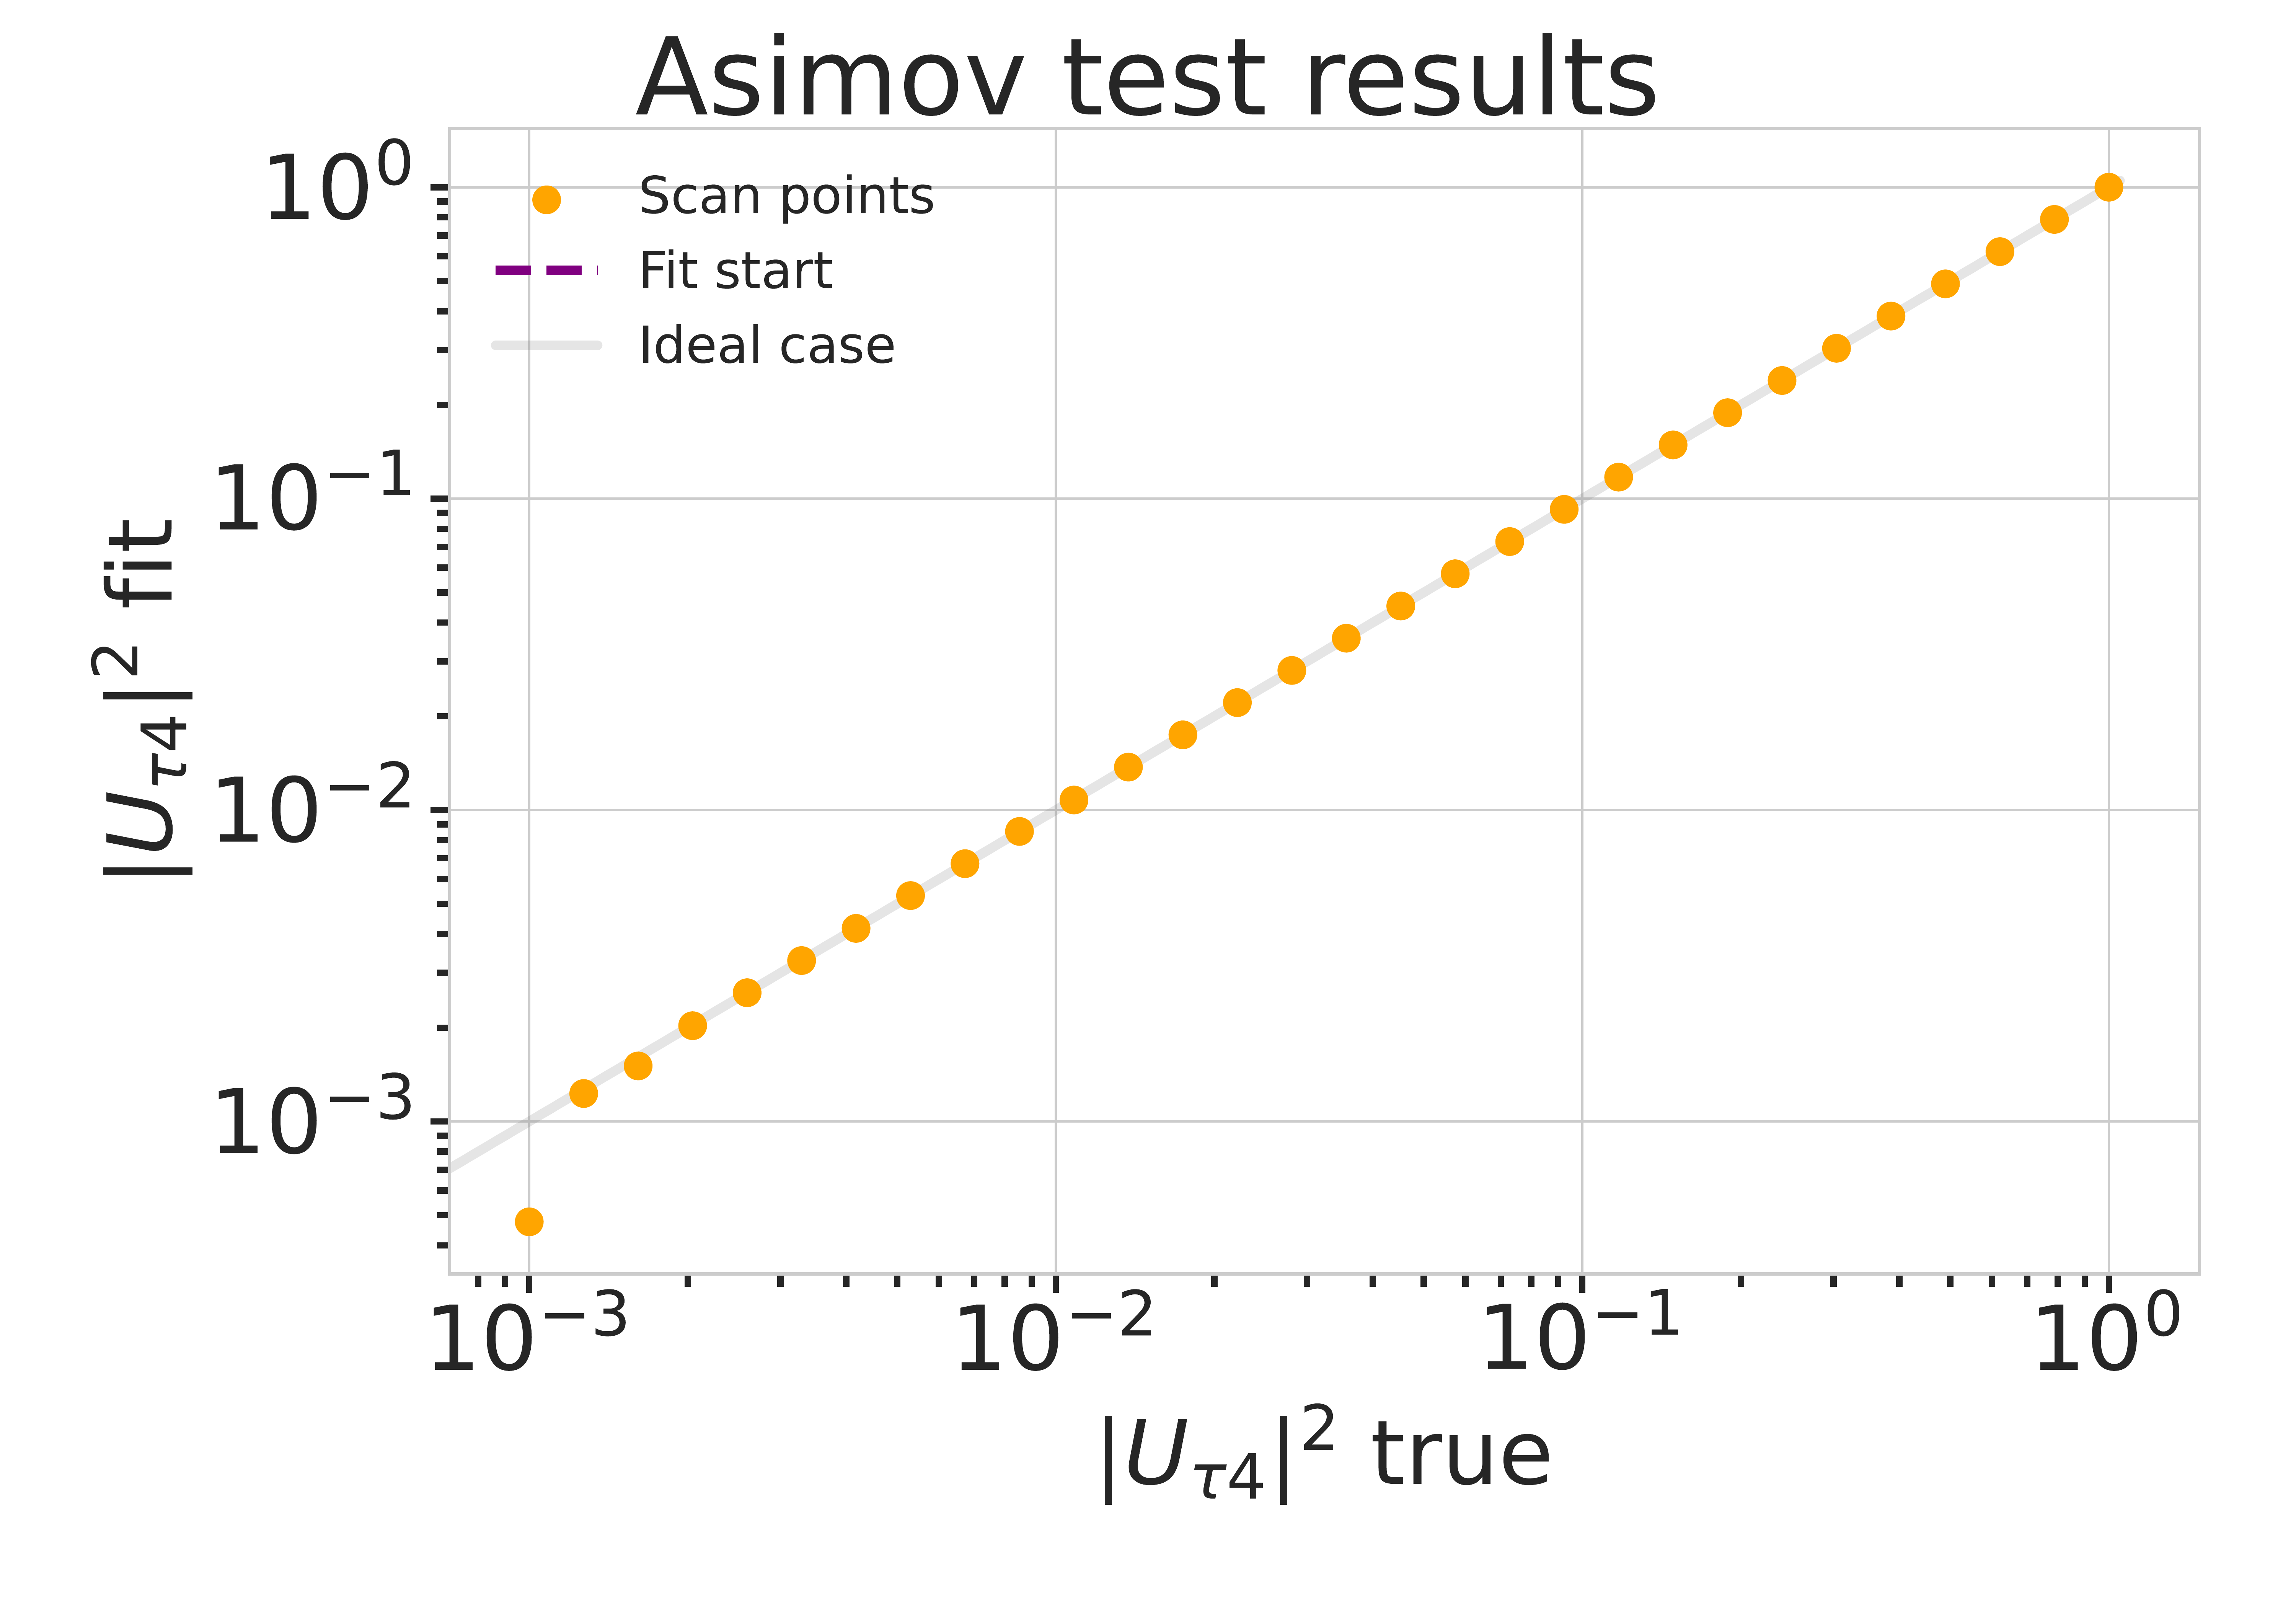
\includegraphics[width=0.49\linewidth]{figures/results/checks/asimov_scan_0.3_GeV-01.png}
%     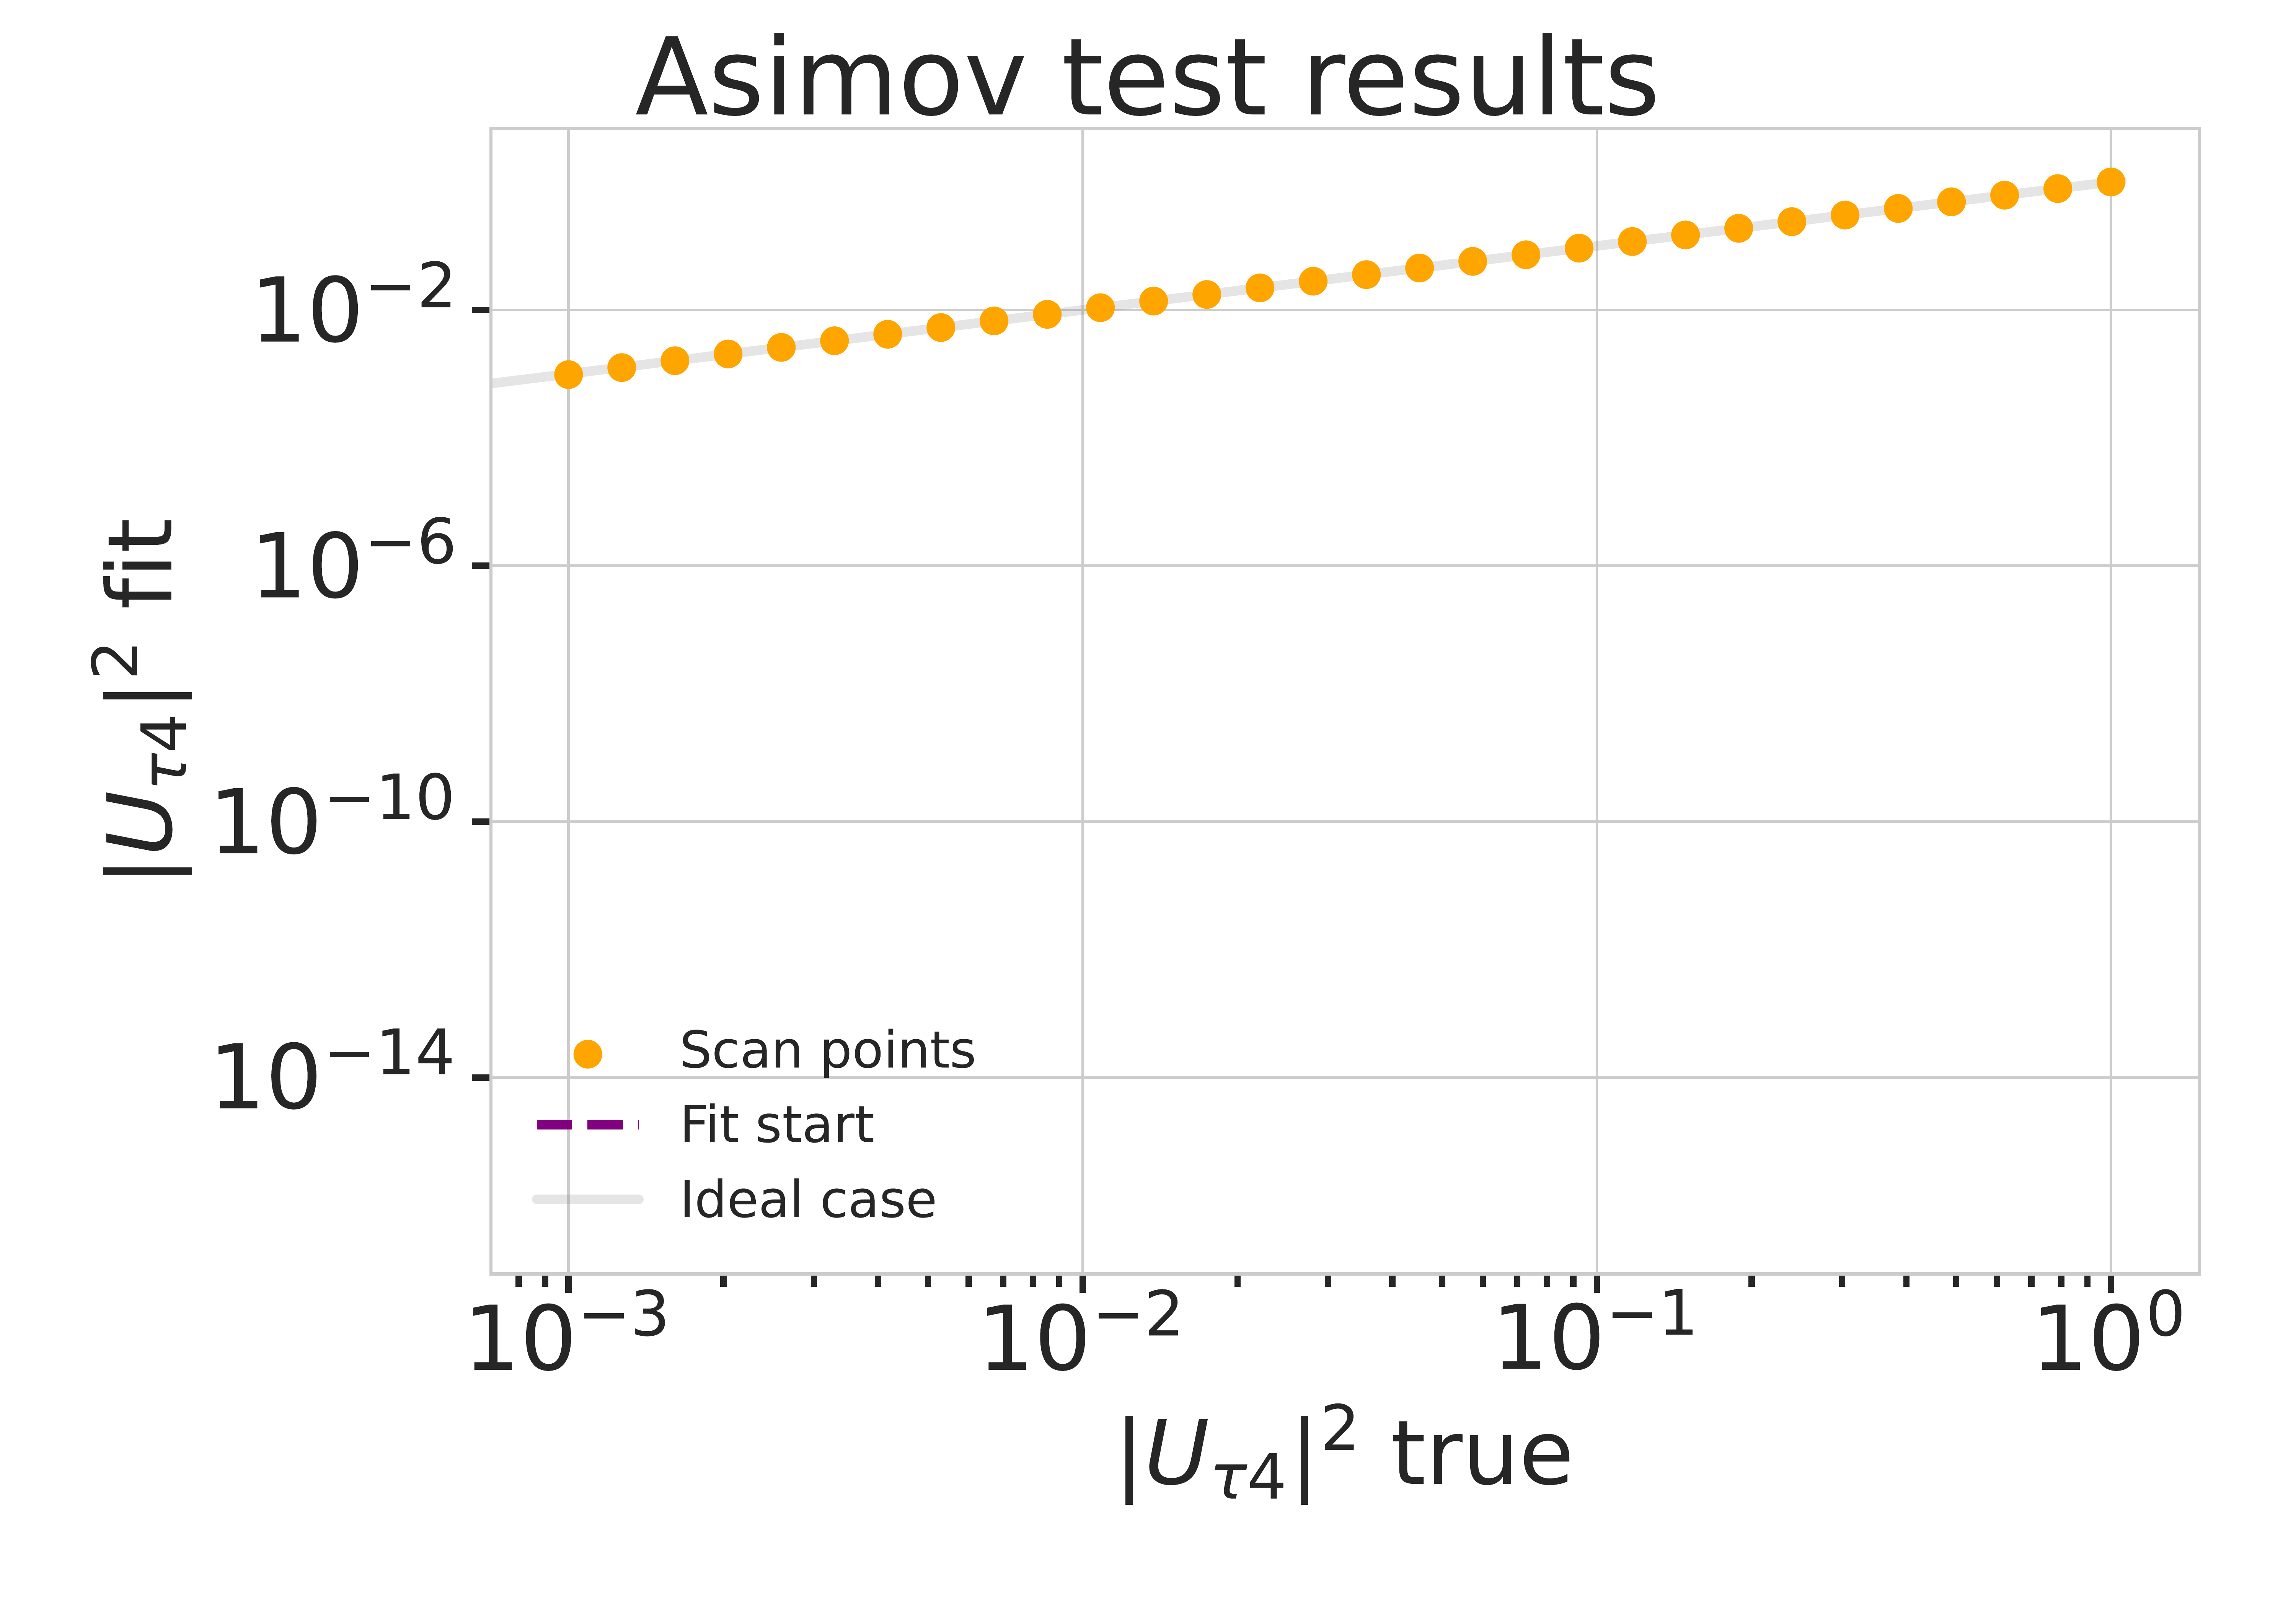
\includegraphics[width=0.49\linewidth]{figures/results/checks/asimov_scan_1.0_GeV-01.png}
% 	\caption[Asimov inject/recover test (\SI{0.3}{\gev}, \SI{1.0}{\gev})]{Asimov inject/recover test for the \SI{0.3}{\gev} (left) and the \SI{1.0}{\gev} (right) mass sets. Mixing values between $10^{-3}$ and $10^{0}$ are injected and fit back with the full analysis chain. The injected parameter is always recovered within the statistical uncertainty.}
%     \labfig{asimov_inject_recover_appendix}
% \end{figure*}


% \section{Sensitivities}

% \begin{figure}[h]
%     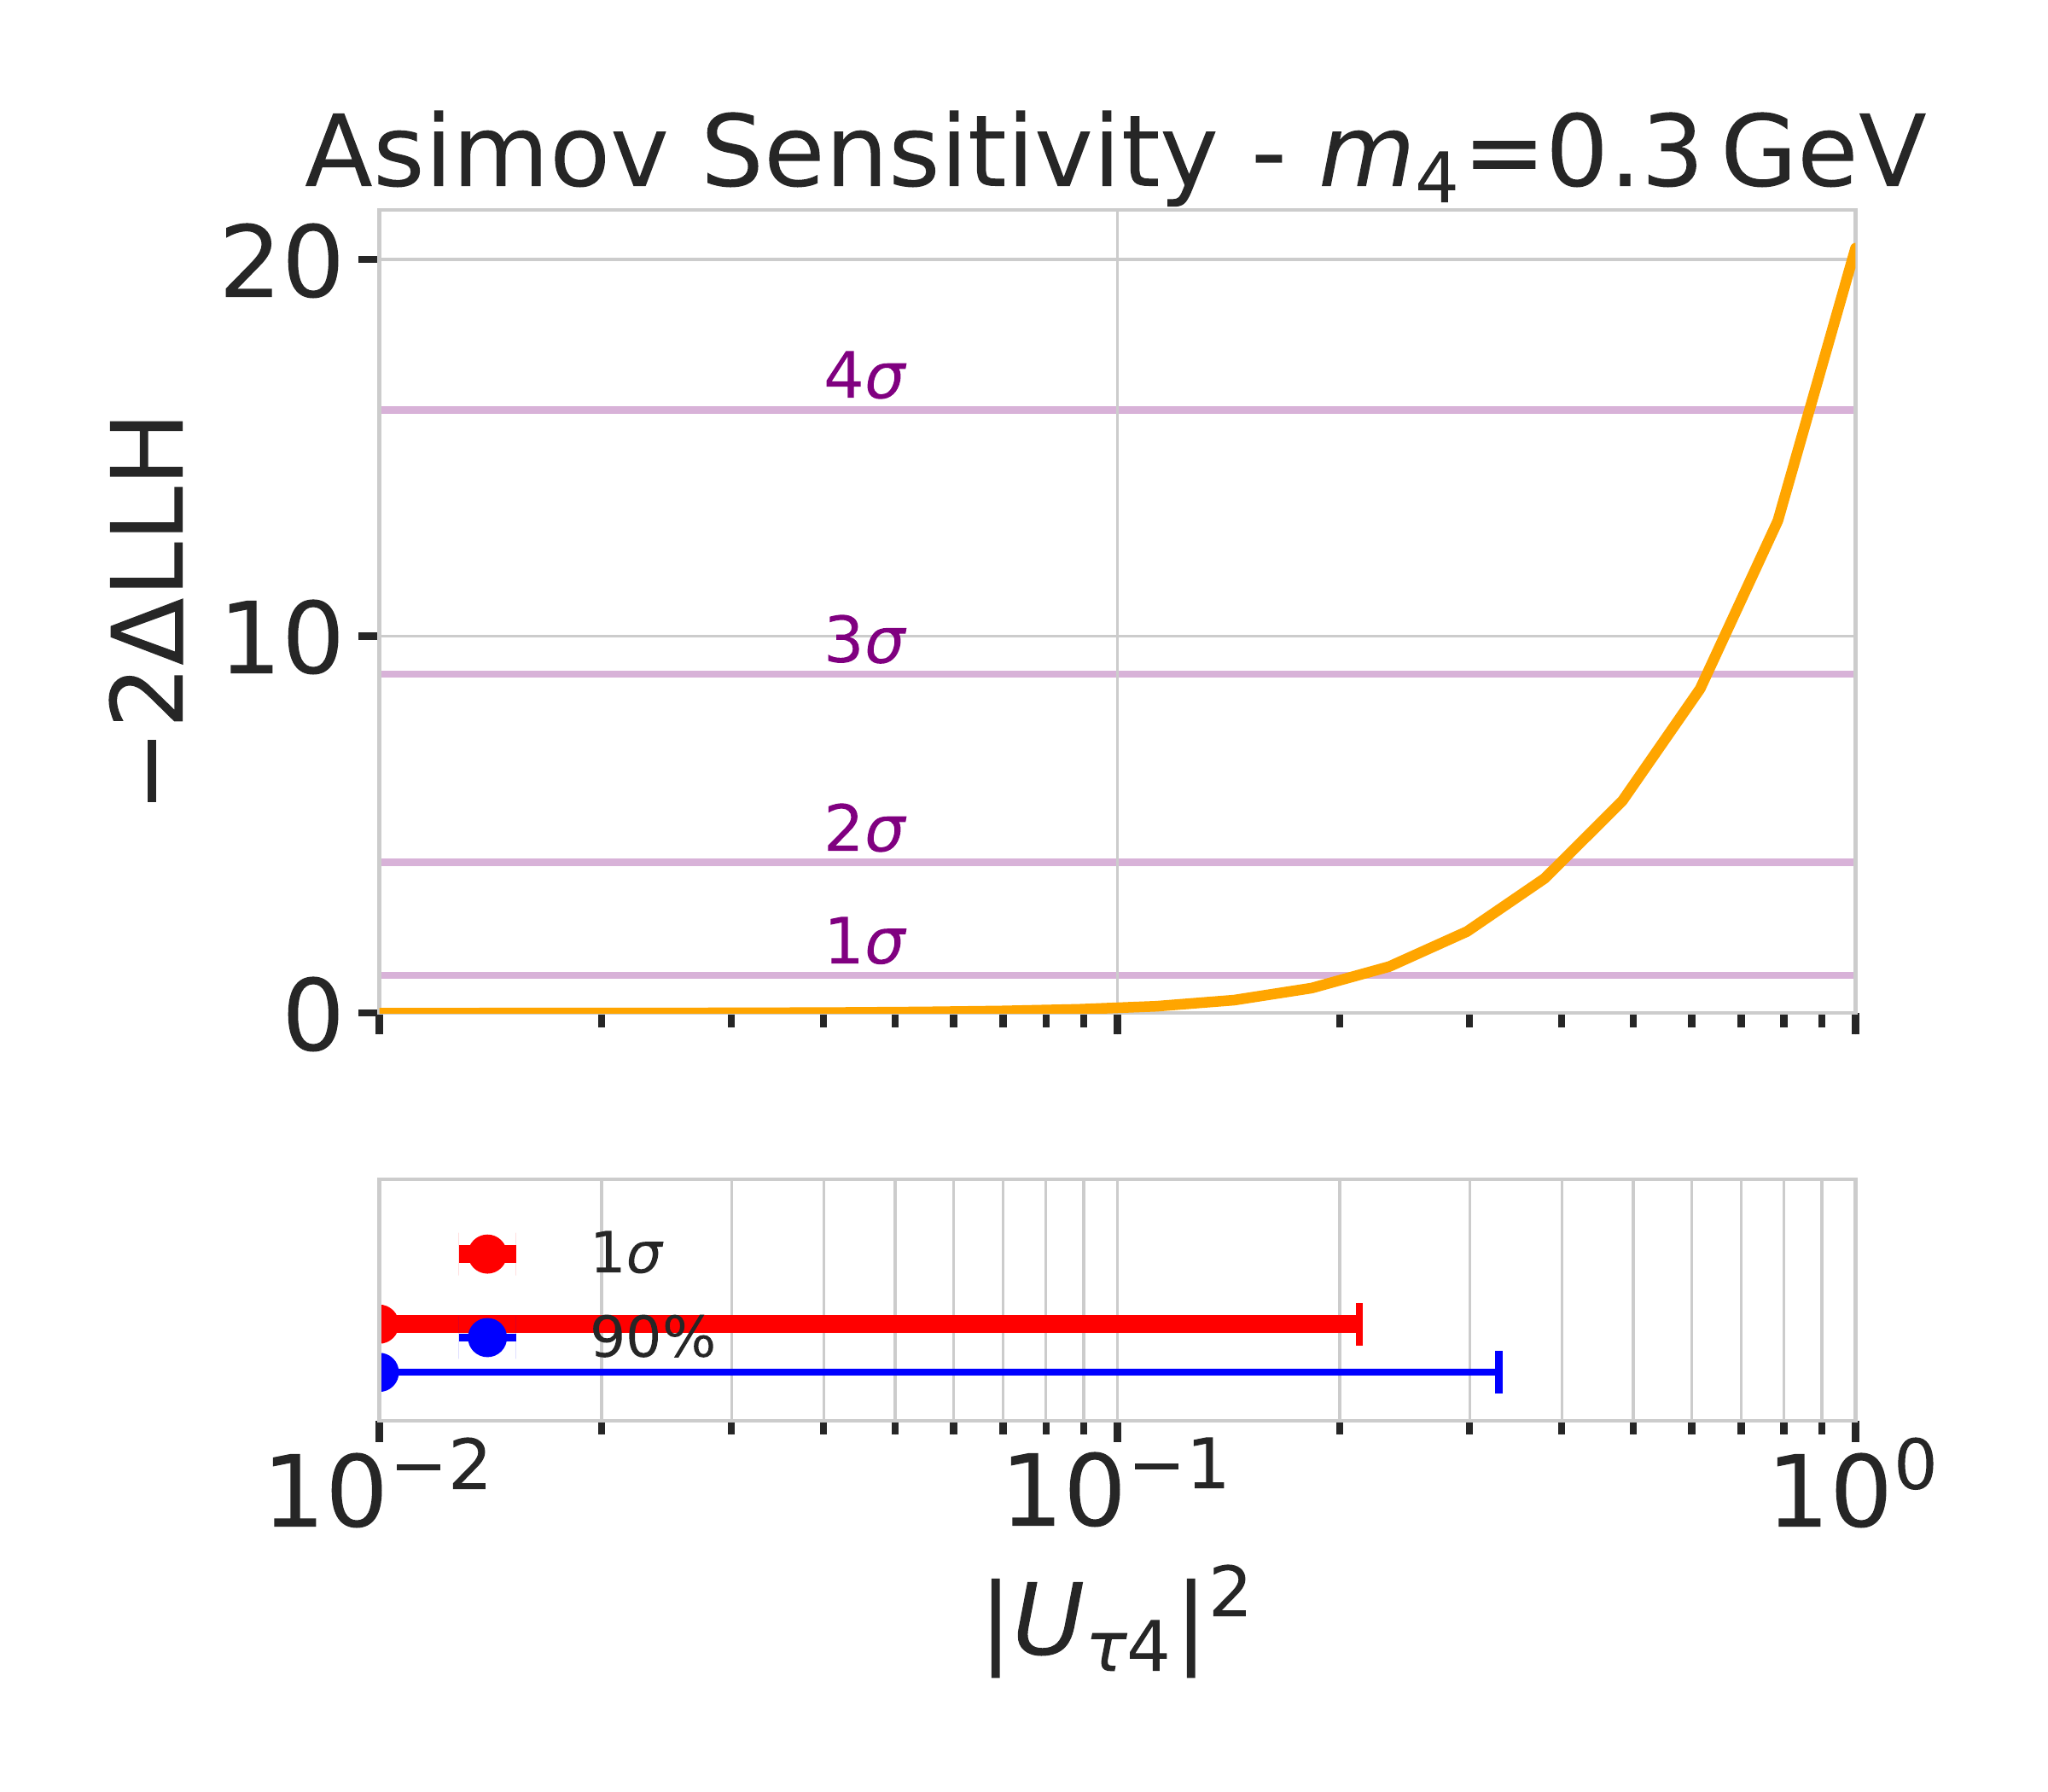
\includegraphics[width=0.49\linewidth]{figures/results/checks/sensitivity_scan_0.3_GeV-1.png}
%     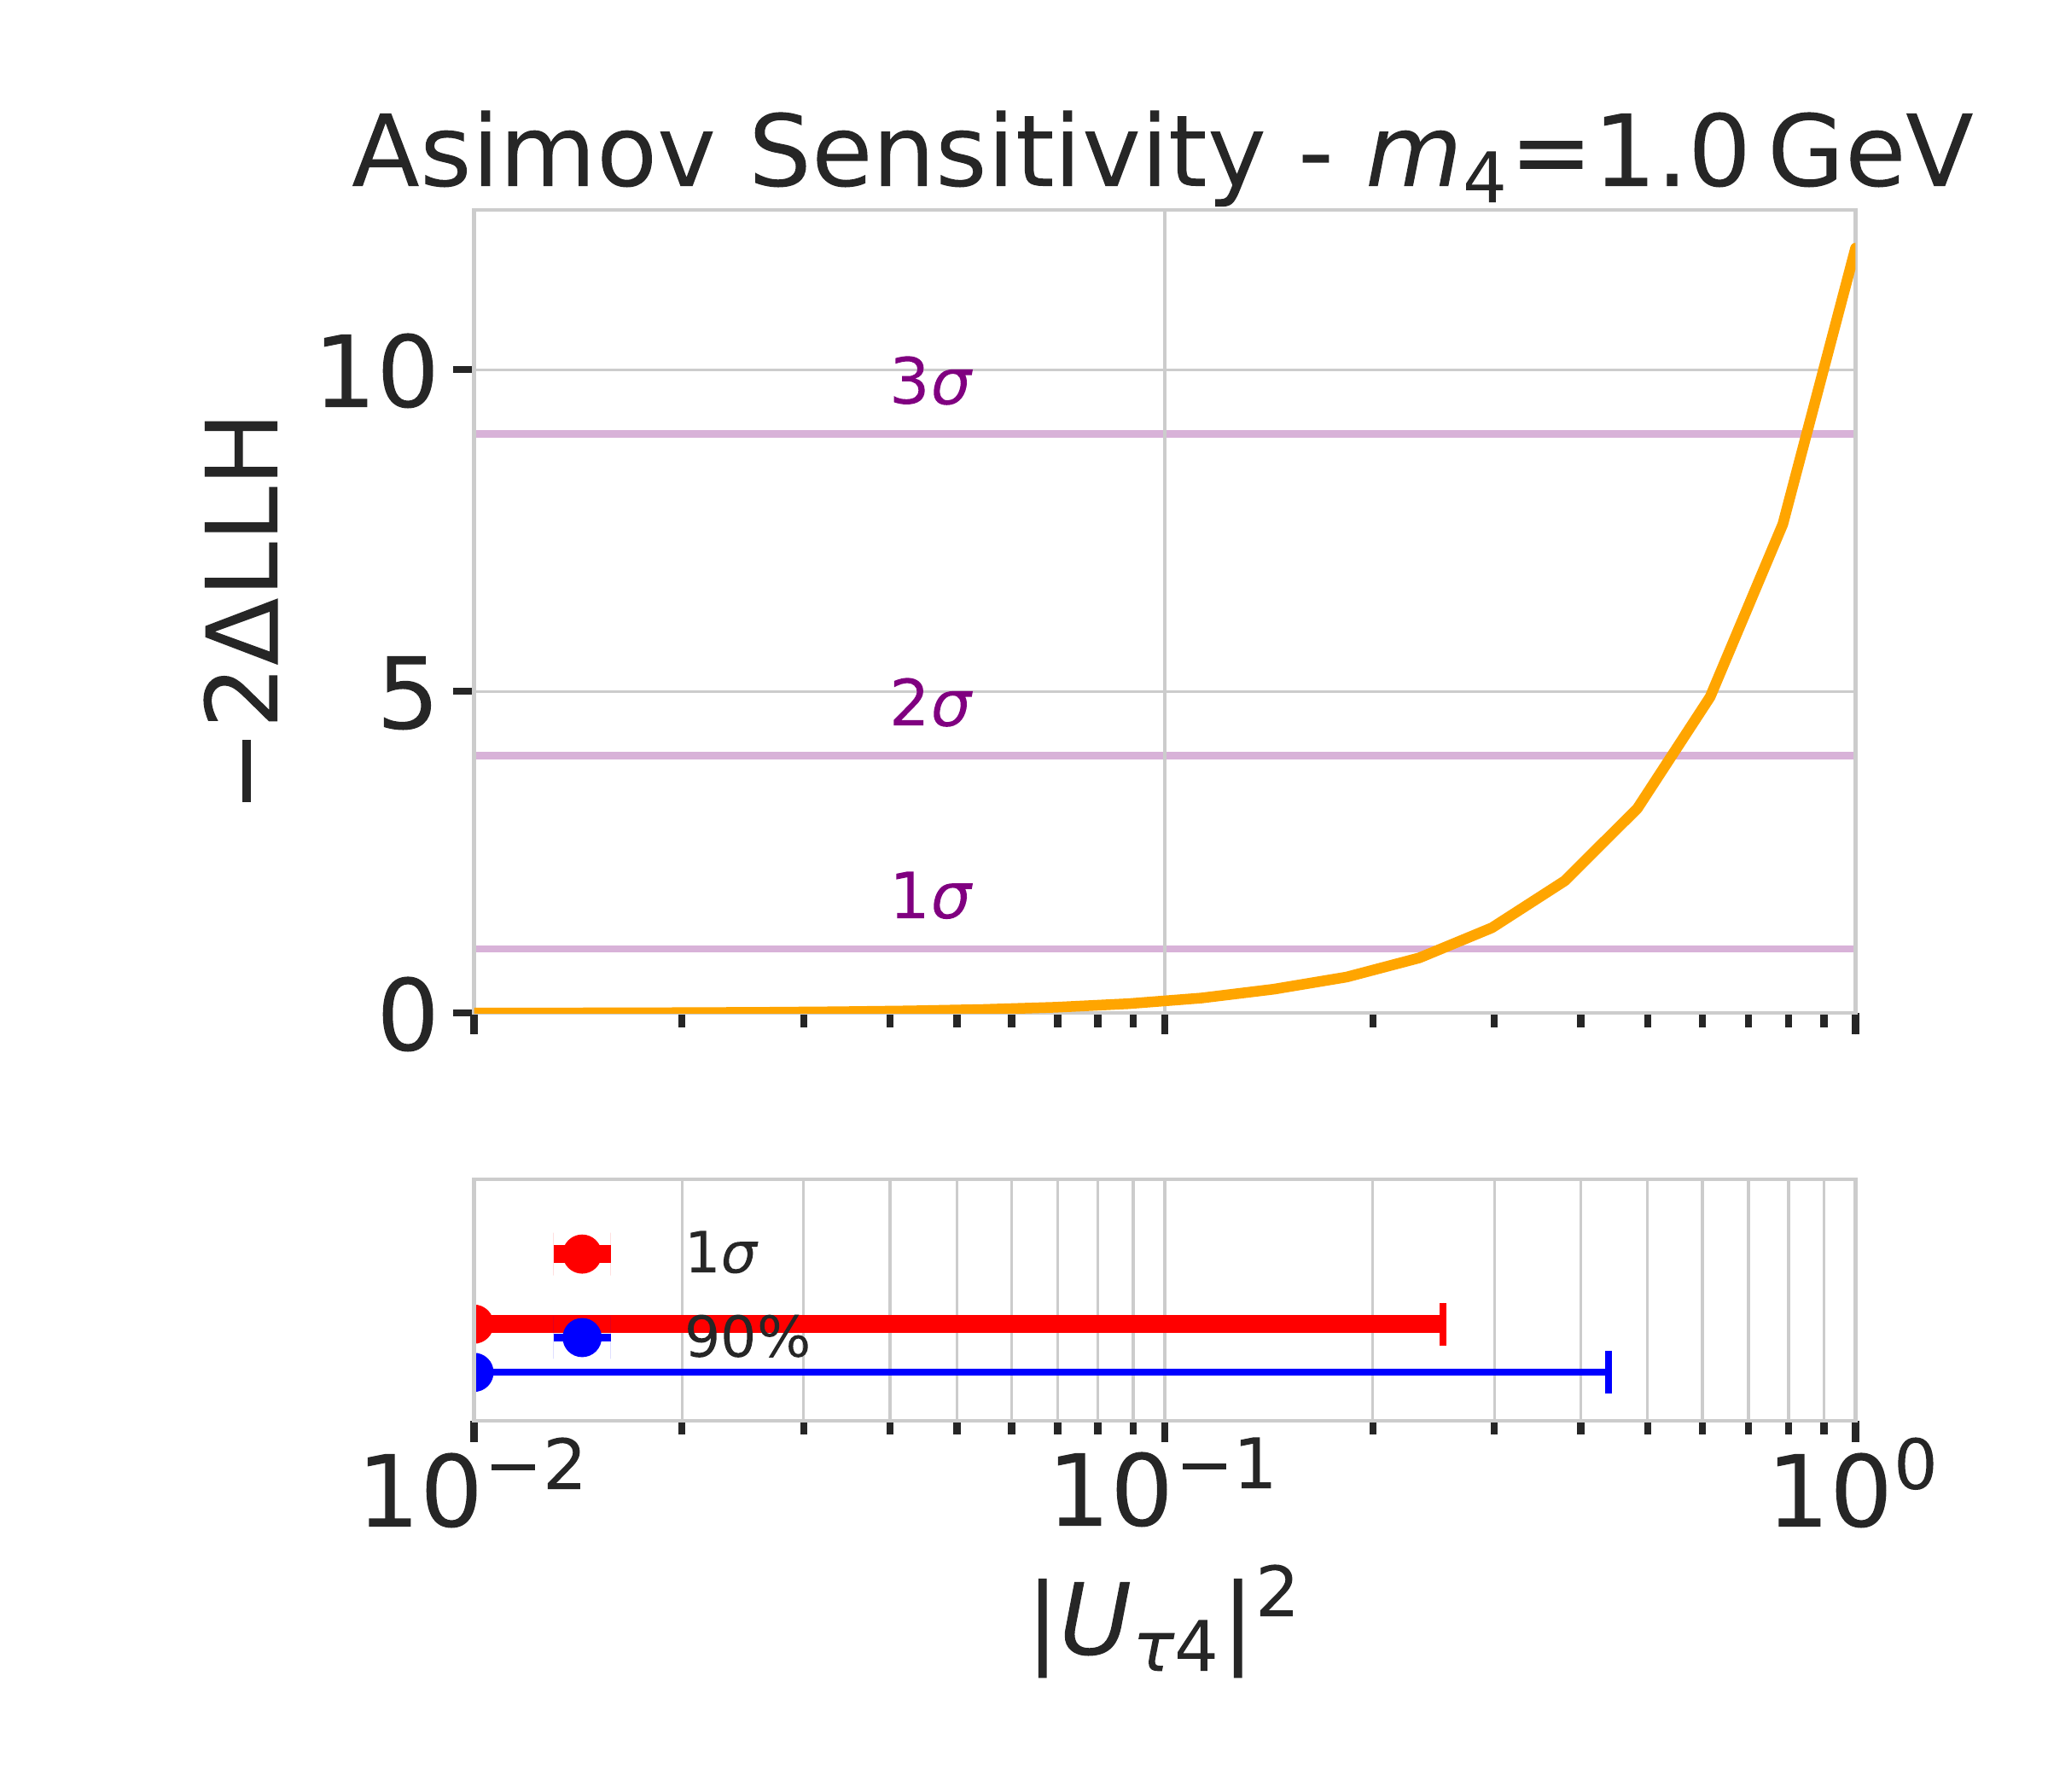
\includegraphics[width=0.49\linewidth]{figures/results/checks/sensitivity_scan_1.0_GeV-1.png}
% 	\caption[Sensitivity scan (\SI{0.3}{\gev}, \SI{1.0}{\gev})]{Sensitivity scan for the \SI{0.3}{\gev} (left) and the \SI{1.0}{\gev} (right) mass sets.}
%     \labfig{sensitivity_scans_appendix}
% \end{figure}



\setchapterstyle{lines}
\chapter{Analysis Results}
\labch{analysis_results}


\section{Best Fit Nuisance Parameters}

\begin{table*}[h]
    \begin{tabular}{ ll lll lll }
    \hline\hline
    \textbf{Parameter} & \textbf{Nominal} & \multicolumn{3}{c}{\textbf{Best Fit}} & \multicolumn{3}{c}{\textbf{Nominal - Best Fit}} \\ 
    & & \textbf{0.3 GeV} & \textbf{0.6 GeV} &  \textbf{1.0 GeV} & \textbf{0.3 GeV} & \textbf{0.6 GeV} &  \textbf{1.0 GeV} \\ 
    \hline\hline
    $|U_{\tau 4}|^2$ & - & 0.003019 & 0.080494 & 0.106141 & - & - & - \\
    $\theta_{23} [\si{\degree}]$ & 47.504700 & 48.117185 & 47.918758 & 48.010986 & $-$0.612485 & $-$0.414058 & $-$0.506286 \\
    $\Delta m^{2}_{31} [\si{\electronvolt^2}]$ & 0.002475  & 0.002454  & 0.002454  & 0.002455  & 0.000020  & 0.000021  & 0.000019  \\
    \hline
    $N_{\nu}$ & 1.000000  & 0.889149  & 0.889055  & 0.889559  & 0.110851  & 0.110945  & 0.110441  \\
    $\Delta \gamma_\nu$ & 0.000000  & $-$0.007926 & $-$0.006692 & $-$0.006596 & 0.007926  & 0.006692  & 0.006596  \\
    $\rm{Barr} \; h_{\pi^+}$ & 0.000000  & $-$0.147475 & $-$0.148481 & $-$0.148059 & 0.147475  & 0.148481  & 0.148059  \\
    $\rm{Barr} \; i_{\pi^+}$ & 0.000000  & 0.475448  & 0.513393  & 0.521626  & $-$0.475448 & $-$0.513393 & $-$0.521626 \\
    $\rm{Barr} \; y_{K^+}$ & 0.000000  & 0.076176  & 0.062893  & 0.057548  & $-$0.076176 & $-$0.062893 & $-$0.057548 \\
    \hline
    $\rm{DIS}$ & 0.000000  & $-$0.248709 & $-$0.223302 & $-$0.215666 & 0.248709  & 0.223302  & 0.215666  \\
    $M_\rm{A,QE}$ & 0.000000  & $-$0.170528 & $-$0.128150 & $-$0.120345 & 0.170528  & 0.128150  & 0.120345  \\
    $M_\rm{A,res}$ & 0.000000  & $-$0.125855 & $-$0.080875 & $-$0.070716 & 0.125855  & 0.080875  & 0.070716  \\
    \hline
    $\epsilon_{\rm{DOM}}$ & 1.000000  & 1.021984  & 1.017789  & 1.016689  & $-$0.021984 & $-$0.017789 & $-$0.016689 \\
    $\rm{hole \, ice} \; p_0$ & 0.101569  & $-$0.161341 & $-$0.161051 & $-$0.160129 & 0.262910  & 0.262620  & 0.261698  \\
    $\rm{hole \, ice} \; p_1$ & $-$0.049344 & $-$0.073701 & $-$0.075596 & $-$0.076261 & 0.024357  & 0.026252  & 0.026917  \\
    $\rm{ice \, absorption}$ & 1.000000  & 0.943261  & 0.942463  & 0.942000  & 0.056739  & 0.057537  & 0.058000  \\
    $\rm{ice \, scattering}$ & 1.050000  & 0.986152  & 0.989289  & 0.989438  & 0.063848  & 0.060711  & 0.060562  \\
    $N_\rm{bfr}$ & 0.000000  & 0.746684  & 0.740255  & 0.736215  & $-$0.746684 & $-$0.740255 & $-$0.736215 \\
    \hline
    \end{tabular}
\caption[xx]{xx}
\labtab{best_fit_parameters}
\end{table*}
\todo{fix caption and design + significant digits to show (ORANGE)}
\todo{maybe show range/prior and then deviation in sigma, or absolute for the ones without prior}
